% **************************************************************************************************************
% A Classic Thesis Style
% An Homage to The Elements of Typographic Style
%
% Copyright (C) 2012 Andr\'e Miede http://www.miede.de
%
% If you like the style then I would appreciate a postcard. My address 
% can be found in the file ClassicThesis.pdf. A collection of the
% postcards I received so far is available online at 
% http://postcards.miede.de
%
% License:
% This program is free software; you can redistribute it and/or modify
% it under the terms of the GNU General Public License as published by
% the Free Software Foundation; either version 2 of the License, or
% (at your option) any later version.
%
% This program is distributed in the hope that it will be useful,
% but WITHOUT ANY WARRANTY; without even the implied warranty of
% MERCHANTABILITY or FITNESS FOR A PARTICULAR PURPOSE.  See the
% GNU General Public License for more details.
%
% You should have received a copy of the GNU General Public License
% along with this program; see the file COPYING.  If not, write to
% the Free Software Foundation, Inc., 59 Temple Place - Suite 330,
% Boston, MA 02111-1307, USA.
%
% **************************************************************************************************************
% Note:
%    * You must not use "u etc. in strings/commands that will be spaced out (use \"u or real umlauts instead)
%    * New enumeration (small caps): \begin{aenumerate} \end{aenumerate}
%    * For margin notes: \marginpar or \graffito{}
%    * Do not use bold fonts in this style, it is designed around them
%    * Use tables as in the examples
%    * See classicthesis-preamble.sty for useful commands
% **************************************************************************************************************
% To Do:
%    * [high] Check this out: http://www.golatex.de/koma-script-warnung-in-verbindung-mit-listings-package-t2058.html
%    * [medium] mathbb in section-titles/chapter-titles => disappears somehow in headlines!!!
% **************************************************************************************************************
\documentclass[ openright,titlepage,numbers=noenddot,headinclude,%,twoside,%1headlines,% letterpaper a4paper
                footinclude=true,cleardoublepage=ehmpty,abstractoff, 
                BCOR=5mm,paper=a4,fontsize=11pt,%11pt,a4paper,%
                ngerman,american,%
                ]{scrreprt}

%********************************************************************
% Note: Make all your adjustments in here
%*******************************************************
% ****************************************************************************************************
% thesis-config.tex 
% Use it at the beginning of your ClassicThesis.tex, or as a LaTeX Preamble 
% in your ClassicThesis.{tex,lyx} with % ****************************************************************************************************
% thesis-config.tex 
% Use it at the beginning of your ClassicThesis.tex, or as a LaTeX Preamble 
% in your ClassicThesis.{tex,lyx} with % ****************************************************************************************************
% thesis-config.tex 
% Use it at the beginning of your ClassicThesis.tex, or as a LaTeX Preamble 
% in your ClassicThesis.{tex,lyx} with \input{thesis-config}
% ****************************************************************************************************

% ****************************************************************************************************
% 1. Personal data and user ad-hoc commands
% ****************************************************************************************************
\usepackage{natbib}

\newcommand{\myTitle}{Verteilte Transaktionssysteme auf Basis des Actor Models\xspace}
%\newcommand{\mySubtitle}{An Homage to The Elements of Typographic Style\xspace}
%\newcommand{\myDegree}{Bachelor of Science (B.Sc)\xspace} 
%\newcommand{\myDegree}{Bachelor of Arts (B.A.)\xspace}
\newcommand{\myDegree}{Master of Science (M.Sc)\xspace}
%\newcommand{\myDegree}{Master of Arts (M.A.)\xspace}
\newcommand{\myName}{Mathias Feitzinger, BSc\xspace}
\newcommand{\myId}{1610738715\xspace}
\newcommand{\myProf}{Prof. (FH) PD Dr. Mario D\"{o}ller\xspace}
\newcommand{\myOtherProf}{Prof. (FH) Dr. Johannes L\"{u}thi\xspace}
\newcommand{\myFaculty}{Web Communication and Information Systems\xspace}
\newcommand{\myUni}{Fachhochschule Kufstein Tirol Bildungs GmbH\xspace}
\newcommand{\myLocation}{Kufstein\xspace}
\newcommand{\myTime}{15. Juni 2018\xspace}
\newcommand{\myVersion}{Version 1.0\xspace}

% ****************************************************************************************************
% 2. Is it a master thesis?
% ****************************************************************************************************
\PassOptionsToPackage{master}{fhkthesis} % uncomment if this is a master thesis 

\interfootnotelinepenalty=10000

% ****************************************************************************************************
% 3. Does the thesis have a lock flag?
% ****************************************************************************************************
%\PassOptionsToPackage{lockflag}{fhkthesis} % uncomment if this thesis has a lock flag 

% ****************************************************************************************************
% 4. Loading some handy packages
% ****************************************************************************************************
% ******************************************************************** 
% Packages with options that might require adjustments
% ******************************************************************** 

%\PassOptionsToPackage{ngerman,american}{babel}   % change this to your language(s)
% Spanish languages need extra options in order to work with this template
%\PassOptionsToPackage{spanish,es-lcroman}{babel}
\usepackage{babel}
\usepackage{nameref}
% ****************************************************************************************************

% ****************************************************************************************************
% 1. Personal data and user ad-hoc commands
% ****************************************************************************************************
\usepackage{natbib}

\newcommand{\myTitle}{Verteilte Transaktionssysteme auf Basis des Actor Models\xspace}
%\newcommand{\mySubtitle}{An Homage to The Elements of Typographic Style\xspace}
%\newcommand{\myDegree}{Bachelor of Science (B.Sc)\xspace} 
%\newcommand{\myDegree}{Bachelor of Arts (B.A.)\xspace}
\newcommand{\myDegree}{Master of Science (M.Sc)\xspace}
%\newcommand{\myDegree}{Master of Arts (M.A.)\xspace}
\newcommand{\myName}{Mathias Feitzinger, BSc\xspace}
\newcommand{\myId}{1610738715\xspace}
\newcommand{\myProf}{Prof. (FH) PD Dr. Mario D\"{o}ller\xspace}
\newcommand{\myOtherProf}{Prof. (FH) Dr. Johannes L\"{u}thi\xspace}
\newcommand{\myFaculty}{Web Communication and Information Systems\xspace}
\newcommand{\myUni}{Fachhochschule Kufstein Tirol Bildungs GmbH\xspace}
\newcommand{\myLocation}{Kufstein\xspace}
\newcommand{\myTime}{15. Juni 2018\xspace}
\newcommand{\myVersion}{Version 1.0\xspace}

% ****************************************************************************************************
% 2. Is it a master thesis?
% ****************************************************************************************************
\PassOptionsToPackage{master}{fhkthesis} % uncomment if this is a master thesis 

\interfootnotelinepenalty=10000

% ****************************************************************************************************
% 3. Does the thesis have a lock flag?
% ****************************************************************************************************
%\PassOptionsToPackage{lockflag}{fhkthesis} % uncomment if this thesis has a lock flag 

% ****************************************************************************************************
% 4. Loading some handy packages
% ****************************************************************************************************
% ******************************************************************** 
% Packages with options that might require adjustments
% ******************************************************************** 

%\PassOptionsToPackage{ngerman,american}{babel}   % change this to your language(s)
% Spanish languages need extra options in order to work with this template
%\PassOptionsToPackage{spanish,es-lcroman}{babel}
\usepackage{babel}
\usepackage{nameref}
% ****************************************************************************************************

% ****************************************************************************************************
% 1. Personal data and user ad-hoc commands
% ****************************************************************************************************
\usepackage{natbib}

\newcommand{\myTitle}{Verteilte Transaktionssysteme auf Basis des Actor Models\xspace}
%\newcommand{\mySubtitle}{An Homage to The Elements of Typographic Style\xspace}
%\newcommand{\myDegree}{Bachelor of Science (B.Sc)\xspace} 
%\newcommand{\myDegree}{Bachelor of Arts (B.A.)\xspace}
\newcommand{\myDegree}{Master of Science (M.Sc)\xspace}
%\newcommand{\myDegree}{Master of Arts (M.A.)\xspace}
\newcommand{\myName}{Mathias Feitzinger, BSc\xspace}
\newcommand{\myId}{1610738715\xspace}
\newcommand{\myProf}{Prof. (FH) PD Dr. Mario D\"{o}ller\xspace}
\newcommand{\myOtherProf}{Prof. (FH) Dr. Johannes L\"{u}thi\xspace}
\newcommand{\myFaculty}{Web Communication and Information Systems\xspace}
\newcommand{\myUni}{Fachhochschule Kufstein Tirol Bildungs GmbH\xspace}
\newcommand{\myLocation}{Kufstein\xspace}
\newcommand{\myTime}{15. Juni 2018\xspace}
\newcommand{\myVersion}{Version 1.0\xspace}

% ****************************************************************************************************
% 2. Is it a master thesis?
% ****************************************************************************************************
\PassOptionsToPackage{master}{fhkthesis} % uncomment if this is a master thesis 

\interfootnotelinepenalty=10000

% ****************************************************************************************************
% 3. Does the thesis have a lock flag?
% ****************************************************************************************************
%\PassOptionsToPackage{lockflag}{fhkthesis} % uncomment if this thesis has a lock flag 

% ****************************************************************************************************
% 4. Loading some handy packages
% ****************************************************************************************************
% ******************************************************************** 
% Packages with options that might require adjustments
% ******************************************************************** 

%\PassOptionsToPackage{ngerman,american}{babel}   % change this to your language(s)
% Spanish languages need extra options in order to work with this template
%\PassOptionsToPackage{spanish,es-lcroman}{babel}
\usepackage{babel}
\usepackage{nameref}
% ****************************************************************************************************
% classicthesis-config.tex 
% formerly known as loadpackages.sty, classicthesis-ldpkg.sty, and classicthesis-preamble.sty 
% Use it at the beginning of your ClassicThesis.tex, or as a LaTeX Preamble 
% in your ClassicThesis.{tex,lyx} with % ****************************************************************************************************
% classicthesis-config.tex 
% formerly known as loadpackages.sty, classicthesis-ldpkg.sty, and classicthesis-preamble.sty 
% Use it at the beginning of your ClassicThesis.tex, or as a LaTeX Preamble 
% in your ClassicThesis.{tex,lyx} with % ****************************************************************************************************
% classicthesis-config.tex 
% formerly known as loadpackages.sty, classicthesis-ldpkg.sty, and classicthesis-preamble.sty 
% Use it at the beginning of your ClassicThesis.tex, or as a LaTeX Preamble 
% in your ClassicThesis.{tex,lyx} with \input{classicthesis-config}
% ****************************************************************************************************  
% If you like the classicthesis, then I would appreciate a postcard. 
% My address can be found in the file ClassicThesis.pdf. A collection 
% of the postcards I received so far is available online at 
% http://postcards.miede.de
% ****************************************************************************************************

% ****************************************************************************************************
% 1. Configure classicthesis for your needs here, e.g., remove "drafting" below 
% in order to deactivate the time-stamp on the pages
% ****************************************************************************************************
\PassOptionsToPackage{eulerchapternumbers,listings,%drafting,
				 pdfspacing,dottedtoc,%floatperchapter,%linedheaders,%
				 subfig,beramono,eulermath,parts}{classicthesis}										
% ********************************************************************
% Available options for classicthesis.sty 
% (see ClassicThesis.pdf for more information):
% drafting
% parts nochapters linedheaders
% eulerchapternumbers beramono eulermath pdfspacing minionprospacing
% tocaligned dottedtoc manychapters
% listings floatperchapter subfig
% ********************************************************************

% ********************************************************************
% Triggers for this config
% ******************************************************************** 
\usepackage{ifthen}
\newboolean{enable-backrefs} % enable backrefs in the bibliography
\setboolean{enable-backrefs}{false} % true false
% ****************************************************************************************************


% ********************************************************************
% 1. Setup, finetuning, and useful commands
% ********************************************************************
\newcounter{dummy} % necessary for correct hyperlinks (to index, bib, etc.)
\newlength{\abcd} % for ab..z string length calculation
\providecommand{\mLyX}{L\kern-.1667em\lower.25em\hbox{Y}\kern-.125emX\@}
\newcommand{\ie}{i.\,e.}
\newcommand{\Ie}{I.\,e.}
\newcommand{\eg}{e.\,g.}
\newcommand{\Eg}{E.\,g.} 
% ****************************************************************************************************


% ****************************************************************************************************
% 2. Loading some handy packages
% ****************************************************************************************************
% ******************************************************************** 
% Packages with options that might require adjustments
% ******************************************************************** 
%\PassOptionsToPackage{latin9}{inputenc}	% latin9 (ISO-8859-9) = latin1+"Euro sign"
\PassOptionsToPackage{utf8}{inputenc}		% utf-8 standard on most modern linux systems
 \usepackage{inputenc}				

%\PassOptionsToPackage{ngerman,american}{babel}   % change this to your language(s)
% Spanish languages need extra options in order to work with this template
%\PassOptionsToPackage{spanish,es-lcroman}{babel}
% \usepackage{babel}					

\PassOptionsToPackage{square,numbers}{natbib}
 \usepackage{natbib}				

\PassOptionsToPackage{fleqn}{amsmath}		 % math environments and more by the AMS 
 \usepackage{amsmath}

\PassOptionsToPackage{doublespacing}{fhkthesis}  % options: abbrev exam big wiwi english master
 \usepackage{fhkthesis}

% ******************************************************************** 
% 4. General useful packages
% ******************************************************************** 
\PassOptionsToPackage{T1}{fontenc} % T2A for cyrillics
	\usepackage{fontenc}     
\usepackage{textcomp} % fix warning with missing font shapes
\usepackage{scrhack} % fix warnings when using KOMA with listings package          
\usepackage{xspace} % to get the spacing after macros right  
\usepackage{mparhack} % get marginpar right
\usepackage{fixltx2e} % fixes some LaTeX stuff 
\PassOptionsToPackage{printonlyused,smaller}{acronym}
	\usepackage{acronym} % nice macros for handling all acronyms in the thesis
%\renewcommand*{\acsfont}[1]{\textssc{#1}} % for MinionPro
%\renewcommand{\bflabel}[1]{{#1}\hfill} % fix the list of acronyms
% ****************************************************************************************************


% ****************************************************************************************************
% 4. Setup floats: tables, (sub)figures, and captions
% ****************************************************************************************************
\usepackage{tabularx} % better tables
	\setlength{\extrarowheight}{3pt} % increase table row height
\newcommand{\tableheadline}[1]{\multicolumn{1}{c}{\spacedlowsmallcaps{#1}}}
\newcommand{\myfloatalign}{\centering} % to be used with each float for alignment
\usepackage{caption}
\captionsetup{format=hang,font=small}
\usepackage{subfig}  
% ****************************************************************************************************


% ****************************************************************************************************
% 5. Setup code listings
% ****************************************************************************************************
\usepackage{listings} 
%\lstset{emph={trueIndex,root},emphstyle=\color{BlueViolet}}%\underbar} % for special keywords
\lstset{language=[LaTeX]Tex,%C++,
    keywordstyle=\color{RoyalBlue},%\bfseries,
    basicstyle=\small\ttfamily,
    %identifierstyle=\color{NavyBlue},
    commentstyle=\color{Green}\ttfamily,
    stringstyle=\rmfamily,
    numbers=none,%left,%
    numberstyle=\scriptsize,%\tiny
    stepnumber=5,
    numbersep=8pt,
    showstringspaces=false,
    breaklines=true,
    frameround=ftff,
    frame=single,
    belowcaptionskip=.75\baselineskip
    %frame=L
} 
% ****************************************************************************************************    		   


% ****************************************************************************************************
% 6. PDFLaTeX, hyperreferences and citation backreferences
% ****************************************************************************************************
% ********************************************************************
% Using PDFLaTeX
% ********************************************************************
\PassOptionsToPackage{pdftex,hyperfootnotes=false,pdfpagelabels}{hyperref}
	\usepackage{hyperref}  % backref linktocpage pagebackref
\pdfcompresslevel=9
\pdfadjustspacing=1 
\PassOptionsToPackage{pdftex}{graphicx}
	\usepackage{graphicx} 

% ********************************************************************
% Setup the style of the backrefs from the bibliography
% (translate the options to any language you use)
% ********************************************************************
\newcommand{\backrefnotcitedstring}{\relax}%(Not cited.)
\newcommand{\backrefcitedsinglestring}[1]{(Cited on page~#1.)}
\newcommand{\backrefcitedmultistring}[1]{(Cited on pages~#1.)}
\ifthenelse{\boolean{enable-backrefs}}%
{%
		\PassOptionsToPackage{hyperpageref}{backref}
		\usepackage{backref} % to be loaded after hyperref package 
		   \renewcommand{\backreftwosep}{ and~} % separate 2 pages
		   \renewcommand{\backreflastsep}{, and~} % separate last of longer list
		   \renewcommand*{\backref}[1]{}  % disable standard
		   \renewcommand*{\backrefalt}[4]{% detailed backref
		      \ifcase #1 %
		         \backrefnotcitedstring%
		      \or%
		         \backrefcitedsinglestring{#2}%
		      \else%
		         \backrefcitedmultistring{#2}%
		      \fi}%
}{\relax}    

% ********************************************************************
% Hyperreferences
% ********************************************************************
\hypersetup{%
    %draft,	% = no hyperlinking at all (useful in b/w printouts)
    colorlinks=true, linktocpage=true, pdfstartpage=3, pdfstartview=FitV,%
    % uncomment the following line if you want to have black links (e.g., for printing)
    %colorlinks=false, linktocpage=false, pdfborder={0 0 0}, pdfstartpage=3, pdfstartview=FitV,% 
    breaklinks=true, pdfpagemode=UseNone, pageanchor=true, pdfpagemode=UseOutlines,%
    plainpages=false, bookmarksnumbered, bookmarksopen=true, bookmarksopenlevel=1,%
    hypertexnames=true, pdfhighlight=/O,%nesting=true,%frenchlinks,%
    urlcolor=webbrown, linkcolor=RoyalBlue, citecolor=webgreen, %pagecolor=RoyalBlue,%
    %urlcolor=Black, linkcolor=Black, citecolor=Black, %pagecolor=Black,%
    pdftitle={\myTitle},%
    pdfauthor={\textcopyright\ \myName, \myUni, \myFaculty},%
    pdfsubject={},%
    pdfkeywords={},%
    pdfcreator={pdfLaTeX},%
    pdfproducer={LaTeX with hyperref and classicthesis}%
}   

% ********************************************************************
% Setup autoreferences
% ********************************************************************
% There are some issues regarding autorefnames
% http://www.ureader.de/msg/136221647.aspx
% http://www.tex.ac.uk/cgi-bin/texfaq2html?label=latexwords
% you have to redefine the makros for the 
% language you use, e.g., american, ngerman
% (as chosen when loading babel/AtBeginDocument)
% ********************************************************************
\makeatletter
\@ifpackageloaded{babel}%
    {%
       \addto\extrasamerican{%
					\renewcommand*{\figureautorefname}{Figure}%
					\renewcommand*{\tableautorefname}{Table}%
					\renewcommand*{\partautorefname}{Part}%
					\renewcommand*{\chapterautorefname}{Chapter}%
					\renewcommand*{\sectionautorefname}{Section}%
					\renewcommand*{\subsectionautorefname}{Section}%
					\renewcommand*{\subsubsectionautorefname}{Section}% 	
				}%
       \addto\extrasngerman{% 
					\renewcommand*{\paragraphautorefname}{Absatz}%
					\renewcommand*{\subparagraphautorefname}{Unterabsatz}%
					\renewcommand*{\footnoteautorefname}{Fu\"snote}%
					\renewcommand*{\FancyVerbLineautorefname}{Zeile}%
					\renewcommand*{\theoremautorefname}{Fragestellung}%
					\renewcommand*{\appendixautorefname}{Anhang}%
					\renewcommand*{\equationautorefname}{Gleichung}%        
					\renewcommand*{\itemautorefname}{Punkt}%
				}%	
			% Fix to getting autorefs for subfigures right (thanks to Belinda Vogt for changing the definition)
			\providecommand{\subfigureautorefname}{\figureautorefname}%  			
    }{\relax}
\makeatother


% ****************************************************************************************************
% 7. Last calls before the bar closes
% ****************************************************************************************************
% ********************************************************************
% Development Stuff
% ********************************************************************
\listfiles
%\PassOptionsToPackage{l2tabu,orthodox,abort}{nag}
%	\usepackage{nag}
%\PassOptionsToPackage{warning, all}{onlyamsmath}
%	\usepackage{onlyamsmath}

% ********************************************************************
% Last, but not least...
% ********************************************************************
\usepackage{classicthesis} 
% ****************************************************************************************************


% ****************************************************************************************************
% 8. Further adjustments (experimental)
% ****************************************************************************************************
% ********************************************************************
% Changing the text area
% ********************************************************************
%\linespread{1.05} % a bit more for Palatino
%\areaset[current]{312pt}{761pt} % 686 (factor 2.2) + 33 head + 42 head \the\footskip
%\setlength{\marginparwidth}{7em}%
%\setlength{\marginparsep}{2em}%

% ********************************************************************
% Using different fonts
% ********************************************************************
%\usepackage[oldstylenums]{kpfonts} % oldstyle notextcomp
%\usepackage[osf]{libertine}
%\usepackage{hfoldsty} % Computer Modern with osf
%\usepackage[light,condensed,math]{iwona}
%\renewcommand{\sfdefault}{iwona}
%\usepackage{lmodern} % <-- no osf support :-(
%\usepackage[urw-garamond]{mathdesign} <-- no osf support :-(
% ****************************************************************************************************

% ****************************************************************************************************  
% If you like the classicthesis, then I would appreciate a postcard. 
% My address can be found in the file ClassicThesis.pdf. A collection 
% of the postcards I received so far is available online at 
% http://postcards.miede.de
% ****************************************************************************************************

% ****************************************************************************************************
% 1. Configure classicthesis for your needs here, e.g., remove "drafting" below 
% in order to deactivate the time-stamp on the pages
% ****************************************************************************************************
\PassOptionsToPackage{eulerchapternumbers,listings,%drafting,
				 pdfspacing,dottedtoc,%floatperchapter,%linedheaders,%
				 subfig,beramono,eulermath,parts}{classicthesis}										
% ********************************************************************
% Available options for classicthesis.sty 
% (see ClassicThesis.pdf for more information):
% drafting
% parts nochapters linedheaders
% eulerchapternumbers beramono eulermath pdfspacing minionprospacing
% tocaligned dottedtoc manychapters
% listings floatperchapter subfig
% ********************************************************************

% ********************************************************************
% Triggers for this config
% ******************************************************************** 
\usepackage{ifthen}
\newboolean{enable-backrefs} % enable backrefs in the bibliography
\setboolean{enable-backrefs}{false} % true false
% ****************************************************************************************************


% ********************************************************************
% 1. Setup, finetuning, and useful commands
% ********************************************************************
\newcounter{dummy} % necessary for correct hyperlinks (to index, bib, etc.)
\newlength{\abcd} % for ab..z string length calculation
\providecommand{\mLyX}{L\kern-.1667em\lower.25em\hbox{Y}\kern-.125emX\@}
\newcommand{\ie}{i.\,e.}
\newcommand{\Ie}{I.\,e.}
\newcommand{\eg}{e.\,g.}
\newcommand{\Eg}{E.\,g.} 
% ****************************************************************************************************


% ****************************************************************************************************
% 2. Loading some handy packages
% ****************************************************************************************************
% ******************************************************************** 
% Packages with options that might require adjustments
% ******************************************************************** 
%\PassOptionsToPackage{latin9}{inputenc}	% latin9 (ISO-8859-9) = latin1+"Euro sign"
\PassOptionsToPackage{utf8}{inputenc}		% utf-8 standard on most modern linux systems
 \usepackage{inputenc}				

%\PassOptionsToPackage{ngerman,american}{babel}   % change this to your language(s)
% Spanish languages need extra options in order to work with this template
%\PassOptionsToPackage{spanish,es-lcroman}{babel}
% \usepackage{babel}					

\PassOptionsToPackage{square,numbers}{natbib}
 \usepackage{natbib}				

\PassOptionsToPackage{fleqn}{amsmath}		 % math environments and more by the AMS 
 \usepackage{amsmath}

\PassOptionsToPackage{doublespacing}{fhkthesis}  % options: abbrev exam big wiwi english master
 \usepackage{fhkthesis}

% ******************************************************************** 
% 4. General useful packages
% ******************************************************************** 
\PassOptionsToPackage{T1}{fontenc} % T2A for cyrillics
	\usepackage{fontenc}     
\usepackage{textcomp} % fix warning with missing font shapes
\usepackage{scrhack} % fix warnings when using KOMA with listings package          
\usepackage{xspace} % to get the spacing after macros right  
\usepackage{mparhack} % get marginpar right
\usepackage{fixltx2e} % fixes some LaTeX stuff 
\PassOptionsToPackage{printonlyused,smaller}{acronym}
	\usepackage{acronym} % nice macros for handling all acronyms in the thesis
%\renewcommand*{\acsfont}[1]{\textssc{#1}} % for MinionPro
%\renewcommand{\bflabel}[1]{{#1}\hfill} % fix the list of acronyms
% ****************************************************************************************************


% ****************************************************************************************************
% 4. Setup floats: tables, (sub)figures, and captions
% ****************************************************************************************************
\usepackage{tabularx} % better tables
	\setlength{\extrarowheight}{3pt} % increase table row height
\newcommand{\tableheadline}[1]{\multicolumn{1}{c}{\spacedlowsmallcaps{#1}}}
\newcommand{\myfloatalign}{\centering} % to be used with each float for alignment
\usepackage{caption}
\captionsetup{format=hang,font=small}
\usepackage{subfig}  
% ****************************************************************************************************


% ****************************************************************************************************
% 5. Setup code listings
% ****************************************************************************************************
\usepackage{listings} 
%\lstset{emph={trueIndex,root},emphstyle=\color{BlueViolet}}%\underbar} % for special keywords
\lstset{language=[LaTeX]Tex,%C++,
    keywordstyle=\color{RoyalBlue},%\bfseries,
    basicstyle=\small\ttfamily,
    %identifierstyle=\color{NavyBlue},
    commentstyle=\color{Green}\ttfamily,
    stringstyle=\rmfamily,
    numbers=none,%left,%
    numberstyle=\scriptsize,%\tiny
    stepnumber=5,
    numbersep=8pt,
    showstringspaces=false,
    breaklines=true,
    frameround=ftff,
    frame=single,
    belowcaptionskip=.75\baselineskip
    %frame=L
} 
% ****************************************************************************************************    		   


% ****************************************************************************************************
% 6. PDFLaTeX, hyperreferences and citation backreferences
% ****************************************************************************************************
% ********************************************************************
% Using PDFLaTeX
% ********************************************************************
\PassOptionsToPackage{pdftex,hyperfootnotes=false,pdfpagelabels}{hyperref}
	\usepackage{hyperref}  % backref linktocpage pagebackref
\pdfcompresslevel=9
\pdfadjustspacing=1 
\PassOptionsToPackage{pdftex}{graphicx}
	\usepackage{graphicx} 

% ********************************************************************
% Setup the style of the backrefs from the bibliography
% (translate the options to any language you use)
% ********************************************************************
\newcommand{\backrefnotcitedstring}{\relax}%(Not cited.)
\newcommand{\backrefcitedsinglestring}[1]{(Cited on page~#1.)}
\newcommand{\backrefcitedmultistring}[1]{(Cited on pages~#1.)}
\ifthenelse{\boolean{enable-backrefs}}%
{%
		\PassOptionsToPackage{hyperpageref}{backref}
		\usepackage{backref} % to be loaded after hyperref package 
		   \renewcommand{\backreftwosep}{ and~} % separate 2 pages
		   \renewcommand{\backreflastsep}{, and~} % separate last of longer list
		   \renewcommand*{\backref}[1]{}  % disable standard
		   \renewcommand*{\backrefalt}[4]{% detailed backref
		      \ifcase #1 %
		         \backrefnotcitedstring%
		      \or%
		         \backrefcitedsinglestring{#2}%
		      \else%
		         \backrefcitedmultistring{#2}%
		      \fi}%
}{\relax}    

% ********************************************************************
% Hyperreferences
% ********************************************************************
\hypersetup{%
    %draft,	% = no hyperlinking at all (useful in b/w printouts)
    colorlinks=true, linktocpage=true, pdfstartpage=3, pdfstartview=FitV,%
    % uncomment the following line if you want to have black links (e.g., for printing)
    %colorlinks=false, linktocpage=false, pdfborder={0 0 0}, pdfstartpage=3, pdfstartview=FitV,% 
    breaklinks=true, pdfpagemode=UseNone, pageanchor=true, pdfpagemode=UseOutlines,%
    plainpages=false, bookmarksnumbered, bookmarksopen=true, bookmarksopenlevel=1,%
    hypertexnames=true, pdfhighlight=/O,%nesting=true,%frenchlinks,%
    urlcolor=webbrown, linkcolor=RoyalBlue, citecolor=webgreen, %pagecolor=RoyalBlue,%
    %urlcolor=Black, linkcolor=Black, citecolor=Black, %pagecolor=Black,%
    pdftitle={\myTitle},%
    pdfauthor={\textcopyright\ \myName, \myUni, \myFaculty},%
    pdfsubject={},%
    pdfkeywords={},%
    pdfcreator={pdfLaTeX},%
    pdfproducer={LaTeX with hyperref and classicthesis}%
}   

% ********************************************************************
% Setup autoreferences
% ********************************************************************
% There are some issues regarding autorefnames
% http://www.ureader.de/msg/136221647.aspx
% http://www.tex.ac.uk/cgi-bin/texfaq2html?label=latexwords
% you have to redefine the makros for the 
% language you use, e.g., american, ngerman
% (as chosen when loading babel/AtBeginDocument)
% ********************************************************************
\makeatletter
\@ifpackageloaded{babel}%
    {%
       \addto\extrasamerican{%
					\renewcommand*{\figureautorefname}{Figure}%
					\renewcommand*{\tableautorefname}{Table}%
					\renewcommand*{\partautorefname}{Part}%
					\renewcommand*{\chapterautorefname}{Chapter}%
					\renewcommand*{\sectionautorefname}{Section}%
					\renewcommand*{\subsectionautorefname}{Section}%
					\renewcommand*{\subsubsectionautorefname}{Section}% 	
				}%
       \addto\extrasngerman{% 
					\renewcommand*{\paragraphautorefname}{Absatz}%
					\renewcommand*{\subparagraphautorefname}{Unterabsatz}%
					\renewcommand*{\footnoteautorefname}{Fu\"snote}%
					\renewcommand*{\FancyVerbLineautorefname}{Zeile}%
					\renewcommand*{\theoremautorefname}{Fragestellung}%
					\renewcommand*{\appendixautorefname}{Anhang}%
					\renewcommand*{\equationautorefname}{Gleichung}%        
					\renewcommand*{\itemautorefname}{Punkt}%
				}%	
			% Fix to getting autorefs for subfigures right (thanks to Belinda Vogt for changing the definition)
			\providecommand{\subfigureautorefname}{\figureautorefname}%  			
    }{\relax}
\makeatother


% ****************************************************************************************************
% 7. Last calls before the bar closes
% ****************************************************************************************************
% ********************************************************************
% Development Stuff
% ********************************************************************
\listfiles
%\PassOptionsToPackage{l2tabu,orthodox,abort}{nag}
%	\usepackage{nag}
%\PassOptionsToPackage{warning, all}{onlyamsmath}
%	\usepackage{onlyamsmath}

% ********************************************************************
% Last, but not least...
% ********************************************************************
\usepackage{classicthesis} 
% ****************************************************************************************************


% ****************************************************************************************************
% 8. Further adjustments (experimental)
% ****************************************************************************************************
% ********************************************************************
% Changing the text area
% ********************************************************************
%\linespread{1.05} % a bit more for Palatino
%\areaset[current]{312pt}{761pt} % 686 (factor 2.2) + 33 head + 42 head \the\footskip
%\setlength{\marginparwidth}{7em}%
%\setlength{\marginparsep}{2em}%

% ********************************************************************
% Using different fonts
% ********************************************************************
%\usepackage[oldstylenums]{kpfonts} % oldstyle notextcomp
%\usepackage[osf]{libertine}
%\usepackage{hfoldsty} % Computer Modern with osf
%\usepackage[light,condensed,math]{iwona}
%\renewcommand{\sfdefault}{iwona}
%\usepackage{lmodern} % <-- no osf support :-(
%\usepackage[urw-garamond]{mathdesign} <-- no osf support :-(
% ****************************************************************************************************

% ****************************************************************************************************  
% If you like the classicthesis, then I would appreciate a postcard. 
% My address can be found in the file ClassicThesis.pdf. A collection 
% of the postcards I received so far is available online at 
% http://postcards.miede.de
% ****************************************************************************************************

% ****************************************************************************************************
% 1. Configure classicthesis for your needs here, e.g., remove "drafting" below 
% in order to deactivate the time-stamp on the pages
% ****************************************************************************************************
\PassOptionsToPackage{eulerchapternumbers,listings,%drafting,
				 pdfspacing,dottedtoc,%floatperchapter,%linedheaders,%
				 subfig,beramono,eulermath,parts}{classicthesis}										
% ********************************************************************
% Available options for classicthesis.sty 
% (see ClassicThesis.pdf for more information):
% drafting
% parts nochapters linedheaders
% eulerchapternumbers beramono eulermath pdfspacing minionprospacing
% tocaligned dottedtoc manychapters
% listings floatperchapter subfig
% ********************************************************************

% ********************************************************************
% Triggers for this config
% ******************************************************************** 
\usepackage{ifthen}
\newboolean{enable-backrefs} % enable backrefs in the bibliography
\setboolean{enable-backrefs}{false} % true false
% ****************************************************************************************************


% ********************************************************************
% 1. Setup, finetuning, and useful commands
% ********************************************************************
\newcounter{dummy} % necessary for correct hyperlinks (to index, bib, etc.)
\newlength{\abcd} % for ab..z string length calculation
\providecommand{\mLyX}{L\kern-.1667em\lower.25em\hbox{Y}\kern-.125emX\@}
\newcommand{\ie}{i.\,e.}
\newcommand{\Ie}{I.\,e.}
\newcommand{\eg}{e.\,g.}
\newcommand{\Eg}{E.\,g.} 
% ****************************************************************************************************


% ****************************************************************************************************
% 2. Loading some handy packages
% ****************************************************************************************************
% ******************************************************************** 
% Packages with options that might require adjustments
% ******************************************************************** 
%\PassOptionsToPackage{latin9}{inputenc}	% latin9 (ISO-8859-9) = latin1+"Euro sign"
\PassOptionsToPackage{utf8}{inputenc}		% utf-8 standard on most modern linux systems
 \usepackage{inputenc}				

%\PassOptionsToPackage{ngerman,american}{babel}   % change this to your language(s)
% Spanish languages need extra options in order to work with this template
%\PassOptionsToPackage{spanish,es-lcroman}{babel}
% \usepackage{babel}					

\PassOptionsToPackage{square,numbers}{natbib}
 \usepackage{natbib}				

\PassOptionsToPackage{fleqn}{amsmath}		 % math environments and more by the AMS 
 \usepackage{amsmath}

\PassOptionsToPackage{doublespacing}{fhkthesis}  % options: abbrev exam big wiwi english master
 \usepackage{fhkthesis}

% ******************************************************************** 
% 4. General useful packages
% ******************************************************************** 
\PassOptionsToPackage{T1}{fontenc} % T2A for cyrillics
	\usepackage{fontenc}     
\usepackage{textcomp} % fix warning with missing font shapes
\usepackage{scrhack} % fix warnings when using KOMA with listings package          
\usepackage{xspace} % to get the spacing after macros right  
\usepackage{mparhack} % get marginpar right
\usepackage{fixltx2e} % fixes some LaTeX stuff 
\PassOptionsToPackage{printonlyused,smaller}{acronym}
	\usepackage{acronym} % nice macros for handling all acronyms in the thesis
%\renewcommand*{\acsfont}[1]{\textssc{#1}} % for MinionPro
%\renewcommand{\bflabel}[1]{{#1}\hfill} % fix the list of acronyms
% ****************************************************************************************************


% ****************************************************************************************************
% 4. Setup floats: tables, (sub)figures, and captions
% ****************************************************************************************************
\usepackage{tabularx} % better tables
	\setlength{\extrarowheight}{3pt} % increase table row height
\newcommand{\tableheadline}[1]{\multicolumn{1}{c}{\spacedlowsmallcaps{#1}}}
\newcommand{\myfloatalign}{\centering} % to be used with each float for alignment
\usepackage{caption}
\captionsetup{format=hang,font=small}
\usepackage{subfig}  
% ****************************************************************************************************


% ****************************************************************************************************
% 5. Setup code listings
% ****************************************************************************************************
\usepackage{listings} 
%\lstset{emph={trueIndex,root},emphstyle=\color{BlueViolet}}%\underbar} % for special keywords
\lstset{language=[LaTeX]Tex,%C++,
    keywordstyle=\color{RoyalBlue},%\bfseries,
    basicstyle=\small\ttfamily,
    %identifierstyle=\color{NavyBlue},
    commentstyle=\color{Green}\ttfamily,
    stringstyle=\rmfamily,
    numbers=none,%left,%
    numberstyle=\scriptsize,%\tiny
    stepnumber=5,
    numbersep=8pt,
    showstringspaces=false,
    breaklines=true,
    frameround=ftff,
    frame=single,
    belowcaptionskip=.75\baselineskip
    %frame=L
} 
% ****************************************************************************************************    		   


% ****************************************************************************************************
% 6. PDFLaTeX, hyperreferences and citation backreferences
% ****************************************************************************************************
% ********************************************************************
% Using PDFLaTeX
% ********************************************************************
\PassOptionsToPackage{pdftex,hyperfootnotes=false,pdfpagelabels}{hyperref}
	\usepackage{hyperref}  % backref linktocpage pagebackref
\pdfcompresslevel=9
\pdfadjustspacing=1 
\PassOptionsToPackage{pdftex}{graphicx}
	\usepackage{graphicx} 

% ********************************************************************
% Setup the style of the backrefs from the bibliography
% (translate the options to any language you use)
% ********************************************************************
\newcommand{\backrefnotcitedstring}{\relax}%(Not cited.)
\newcommand{\backrefcitedsinglestring}[1]{(Cited on page~#1.)}
\newcommand{\backrefcitedmultistring}[1]{(Cited on pages~#1.)}
\ifthenelse{\boolean{enable-backrefs}}%
{%
		\PassOptionsToPackage{hyperpageref}{backref}
		\usepackage{backref} % to be loaded after hyperref package 
		   \renewcommand{\backreftwosep}{ and~} % separate 2 pages
		   \renewcommand{\backreflastsep}{, and~} % separate last of longer list
		   \renewcommand*{\backref}[1]{}  % disable standard
		   \renewcommand*{\backrefalt}[4]{% detailed backref
		      \ifcase #1 %
		         \backrefnotcitedstring%
		      \or%
		         \backrefcitedsinglestring{#2}%
		      \else%
		         \backrefcitedmultistring{#2}%
		      \fi}%
}{\relax}    

% ********************************************************************
% Hyperreferences
% ********************************************************************
\hypersetup{%
    %draft,	% = no hyperlinking at all (useful in b/w printouts)
    colorlinks=true, linktocpage=true, pdfstartpage=3, pdfstartview=FitV,%
    % uncomment the following line if you want to have black links (e.g., for printing)
    %colorlinks=false, linktocpage=false, pdfborder={0 0 0}, pdfstartpage=3, pdfstartview=FitV,% 
    breaklinks=true, pdfpagemode=UseNone, pageanchor=true, pdfpagemode=UseOutlines,%
    plainpages=false, bookmarksnumbered, bookmarksopen=true, bookmarksopenlevel=1,%
    hypertexnames=true, pdfhighlight=/O,%nesting=true,%frenchlinks,%
    urlcolor=webbrown, linkcolor=RoyalBlue, citecolor=webgreen, %pagecolor=RoyalBlue,%
    %urlcolor=Black, linkcolor=Black, citecolor=Black, %pagecolor=Black,%
    pdftitle={\myTitle},%
    pdfauthor={\textcopyright\ \myName, \myUni, \myFaculty},%
    pdfsubject={},%
    pdfkeywords={},%
    pdfcreator={pdfLaTeX},%
    pdfproducer={LaTeX with hyperref and classicthesis}%
}   

% ********************************************************************
% Setup autoreferences
% ********************************************************************
% There are some issues regarding autorefnames
% http://www.ureader.de/msg/136221647.aspx
% http://www.tex.ac.uk/cgi-bin/texfaq2html?label=latexwords
% you have to redefine the makros for the 
% language you use, e.g., american, ngerman
% (as chosen when loading babel/AtBeginDocument)
% ********************************************************************
\makeatletter
\@ifpackageloaded{babel}%
    {%
       \addto\extrasamerican{%
					\renewcommand*{\figureautorefname}{Figure}%
					\renewcommand*{\tableautorefname}{Table}%
					\renewcommand*{\partautorefname}{Part}%
					\renewcommand*{\chapterautorefname}{Chapter}%
					\renewcommand*{\sectionautorefname}{Section}%
					\renewcommand*{\subsectionautorefname}{Section}%
					\renewcommand*{\subsubsectionautorefname}{Section}% 	
				}%
       \addto\extrasngerman{% 
					\renewcommand*{\paragraphautorefname}{Absatz}%
					\renewcommand*{\subparagraphautorefname}{Unterabsatz}%
					\renewcommand*{\footnoteautorefname}{Fu\"snote}%
					\renewcommand*{\FancyVerbLineautorefname}{Zeile}%
					\renewcommand*{\theoremautorefname}{Fragestellung}%
					\renewcommand*{\appendixautorefname}{Anhang}%
					\renewcommand*{\equationautorefname}{Gleichung}%        
					\renewcommand*{\itemautorefname}{Punkt}%
				}%	
			% Fix to getting autorefs for subfigures right (thanks to Belinda Vogt for changing the definition)
			\providecommand{\subfigureautorefname}{\figureautorefname}%  			
    }{\relax}
\makeatother


% ****************************************************************************************************
% 7. Last calls before the bar closes
% ****************************************************************************************************
% ********************************************************************
% Development Stuff
% ********************************************************************
\listfiles
%\PassOptionsToPackage{l2tabu,orthodox,abort}{nag}
%	\usepackage{nag}
%\PassOptionsToPackage{warning, all}{onlyamsmath}
%	\usepackage{onlyamsmath}

% ********************************************************************
% Last, but not least...
% ********************************************************************
\usepackage{classicthesis} 
% ****************************************************************************************************


% ****************************************************************************************************
% 8. Further adjustments (experimental)
% ****************************************************************************************************
% ********************************************************************
% Changing the text area
% ********************************************************************
%\linespread{1.05} % a bit more for Palatino
%\areaset[current]{312pt}{761pt} % 686 (factor 2.2) + 33 head + 42 head \the\footskip
%\setlength{\marginparwidth}{7em}%
%\setlength{\marginparsep}{2em}%

% ********************************************************************
% Using different fonts
% ********************************************************************
%\usepackage[oldstylenums]{kpfonts} % oldstyle notextcomp
%\usepackage[osf]{libertine}
%\usepackage{hfoldsty} % Computer Modern with osf
%\usepackage[light,condensed,math]{iwona}
%\renewcommand{\sfdefault}{iwona}
%\usepackage{lmodern} % <-- no osf support :-(
%\usepackage[urw-garamond]{mathdesign} <-- no osf support :-(
% ****************************************************************************************************


% ********************************************************************
% Hyphenation
% ********************************************************************
%\hyphenation{put special hyphenation here}

% ********************************************************************
% GO!GO!GO! MOVE IT!
% ********************************************************************
\begin{document}
\frenchspacing
\raggedbottom
\selectlanguage{ngerman} % american ngerman
\pagenumbering{roman}
\pagestyle{plain}
% ********************************************************************
% Frontmatter
% ********************************************************************
%*******************************************************
% Titlepage
%*******************************************************
%%%
%%% title page (german)
%%%
\thispagestyle{empty}
\pdfbookmark[0]{Titelblatt}{title}
\begin{titlepage}

  % If printed on two sides, center the title page
  \condTWOSIDE{\changetext{}{19mm}{}{19mm}{}}

  \vspace{1cm}
  \begin{center}
    \hfill
\includegraphics[width=4.5cm]{gfx/logo_fh-kufstein} \\ 
  \end{center}
  \vfill

  \begin{center}
    \LARGE \textbf{\myTitle}
  \end{center} 
  \vfill

  \begin{center}
    %\condMASTER{\Large Masterarbeit}{\Large Bachelorarbeit}
    \ifthenelse{\boolean{@master}}{\Large Masterarbeit}{\Large Bachelorarbeit}
  \end{center}
  \vfill

  \begin{center}
    \Large{zur Erlangung des akademischen Grades}
  \end{center}
  \vfill

  \begin{center}
    \LARGE \textbf{\myDegree}
  \end{center}
  \vfill

  \begin{center}
    \large Eingereicht bei:\\ 
    \vspace{0.1cm}
    \large \textbf{\myUni}\\
    \vspace{0.1cm}
    \large \textbf{\myFaculty}
  \end{center}
  \vfill

  \begin{center}
    \large Verfasser/in:\\
    \vspace{0.1cm}
    \large \textbf{\myName}\\
    \vspace{0.1cm}
    \large \textbf{\myId}\\
  \end{center}
  \vfill

  \begin{center}
    \begin{tabular}{lll}
      Erstgutachter  & : & \myProf \\
      \condMASTER{Zweitgutachter & : & \myOtherProf}
    \end{tabular}
  \end{center} 
  \vfill

  \begin{center}
    \large Abgabedatum: \\
    \vspace{0.1cm}
    \large \textbf{\myTime}
  \end{center} 
%  \vfill
%  \vfill

%  \begin{center}
%    \large \selectedthesisnumber \\
%  \end{center}

  % If printed on two sides, center the title page
  \condTWOSIDE{\changetext{}{-19mm}{}{-19mm}{}}

\end{titlepage}

\condTWOSIDE{\thispagestyle{empty}

\hfill

\vfill

\noindent\myName: \textit{\myTitle,} \myDegree, \textcopyright\ \myTime

%\bigskip
%
%\noindent\spacedlowsmallcaps{Supervisors}: \\
%\myProf \\
%\myOtherProf \\ 
%\mySupervisor
%
%\medskip
%
%\noindent\spacedlowsmallcaps{Location}: \\
%\myLocation
%
%\medskip
%
%\noindent\spacedlowsmallcaps{Time Frame}: \\
%\myTime
}
\cleardoublepage%*******************************************************
% Declaration
%*******************************************************
\refstepcounter{dummy}
\pdfbookmark[1]{Eidesstattliche Erkl\"{a}rung}{eidesstattliche erkl\"{a}rung}
\chapter*{Eidesstattliche Erkl\"{a}rung}
\thispagestyle{empty}

Ich erkl\"{a}re hiermit, dass ich die vorliegende Masterarbeit selbst\"{a}ndig und ohne fremde Hilfsmittel verfasst und in der Bearbeitung und Abfassung keine anderen als die angegebenen Quellen oder Hilfsmittel benutzt sowie w\"{o}rtliche und sinngem\"{a}{\ss}e Zitate als solche gekennzeichnet habe. Die vorliegende Masterarbeit wurde nicht anderweitig f\"{u}r Pr\"{u}fungszwecke vorgelegt.
\bigskip
 
\noindent\textit{\myLocation, den \myTime}

\smallskip

\begin{flushright}
  \begin{tabular}{m{5cm}}
    \\ \hline
    \centering\myName \\
  \end{tabular}
\end{flushright}

\condLOCK{\cleardoublepage%*******************************************************
% Declaration
%*******************************************************
\refstepcounter{dummy}
\pdfbookmark[1]{Sperrvermerk}{Sperrvermerk}
\chapter*{Sperrvermerk}
\thispagestyle{empty}

Ich habe die Sperrung meiner \ifthenelse{\boolean{@master}}{Masterarbeit}{Bachelorarbeit} beantragt, welche von der Studiengangsleitung genehmigt wurde.
\bigskip
 
\noindent\textit{\myLocation, den \myTime}

\smallskip

\begin{flushright}
  \begin{tabular}{m{5cm}}
    \\ \hline
    \centering\myName \\
  \end{tabular}
\end{flushright}
}
\condDOUBLESPACING{\onehalfspacing}
\cleardoublepage%*******************************************************
% Abstract
%*******************************************************
\pdfbookmark[1]{Zusammenfassung}{Zusammenfassung}
\chapter*{Zusammenfassung}
Das Entwerfen von Softwarearchitekturen, welche modernsten Anforderungen entsprechen sollen, ist eine komplexe und schwierige Aufgabe. Eine Möglichkeit Verteilte Software zu entwerfen bietet das Actor Model, welches im Zuge dieser Arbeit ausführlich diskutiert wird. Das in \cite{Hewitt1973AIntelligence} vorgestellte \textit{Actor-Model} wurde als Programmiermodel für parallelisierte Softwareentwicklung entworfen. Die Eigenschaften dieses Models wie die Nachrichtenorientierung oder die Datenisolierung, sind auch bestens als Grundlage für verteilte Softwarearchitekturen geeignet. \\
Um Softwareanwendungen zu entwickeln, welche den herausfordernden aktuellen Anforderungen gerecht werden, sollte die Architektur der Software verschiedene grundlegende Eigenschaften aufweisen. Unter anderem ist hier das \textit{Reactive Manifesto}, eine Grundlage moderner Softwarearchitektur, zu nennen. 
\\
Eine häufige Anforderung von Business Anwendungen ist die Konsistenz und Dauerhaftigkeit der verarbeiteten Daten. Die Verteilung solcher verteilten und Datenhaltenden Systeme birgt einige Probleme wie das CAP-Theorem \citep{gilbertPerspectiveCAPTheorem2012}. 
\\
Im Zuge der Masterarbeit, wurde aufgrund der theoretischen Auseinandersetzung mit den drei Hauptthemen Actor Model, Transaktionssyteme und Verteilte Systeme ein Anforderungskatalog erstellt, der die typischen Anwendungsgebiete dieser drei Themen zusammenfasst. Der Anforderungskatalog beschreibt das fiktive Flugbuchungssystem \textit{TyrolSky}. Dabei liegt der Schwerpunkt der Implementierung auf der Verteilung der gesamten Anwendung, ohne dabei Dateninkonsistenzen bei den Anwendungsspezifischen Daten zuzulassen. 
\\
Die Implementierung erfolgt auf Basis des Actor Framworks \textit{Akka.net} \citep{Akka.netCommunityAkka.NETDocumentation}. Die Implementierte Lösung bietet vier verschiedene Komponenten welche alle mehrfach instanziiert werden. Die Verteilung der Daten innerhalb dieser Komponenten wird von der Software automatisch vorgenommen. 
\\
Die Arbeit konnte zeigen, dass das Actor-Model für die Entwicklung von verteilen Systemen geeignet ist. Das Entwerfen von verteilten Systemen mit Transaktionsdaten bleibt aber eine Herausforderung. Bei der bewältigung dieser Hürden, kann das \textit{Actor-Model} den Entwickler unterstützen.

\cleardoublepage

\cleardoublepage%*******************************************************
% Abstract
%*******************************************************
%\renewcommand{\abstractname}{Abstract}
\pdfbookmark[1]{Abstract}{Abstract}

\chapter*{Abstract}
\selectlanguage{american} % american ngerman
Designing software architectures to meet the latest requirements is a complex and difficult task. One possibility to design distributed software is offered by the actor-model, which is discussed in detail in the context of this work. TheActor-Model was designed as a programming model for parallel software development \citep{hewitt1973session}. The characteristics of this model, such as message orientation or data isolation, are ideally suited as a basis for distributed software architectures. \\
In order to develop software applications, the architecture of the software should have various elementary properties in order to meet current requirements. Among other things, the Reactive Manifesto (\cite{reactiveManifesto}) provides a basis for a modern software architecture. 
A frequent requirement of business applications is the consistency and durability of the processed data. The distribution of such systems has some problems, such as the CAP theorem \citep{gilbertPerspectiveCAPTheorem2012}. \\
In the scope of this master thesis, based on the theoretical examination of the three main topics actor-model, transaction-systems and distributed-systems, a set of requirements was created which summarizes the typical fields of application of these three topics. The fictional flight booking system \textit{TyrolSky} is used as an application example. The implementation is focused on distributing the entire application without allowing data inconsistencies in the application specific data. \\
The implementation is based on the actor-framwork \textit{Akka.NET} (\cite{Akka.NETCommunityAkka.NETDocumentation}). This implemented solution offers four different components, all of which are instantiated several times. The software automatically distributes the data within these components.
The work showed that the actor-model is suitable for the development of distributed systems. Designing distributed systems with transaction data remains a challenge but the Actor-Model can be used to support easier handling of this.


\cleardoublepage
\selectlanguage{ngerman} % american ngerman
\pagestyle{scrheadings}
\cleardoublepage%*******************************************************
% Table of Contents
%*******************************************************
%\phantomsection
\refstepcounter{dummy}
\pdfbookmark[1]{\contentsname}{tableofcontents}
\setcounter{tocdepth}{2} % <-- 2 includes up to subsections in the ToC
\setcounter{secnumdepth}{3} % <-- 3 numbers up to subsubsections
\manualmark
\markboth{\spacedlowsmallcaps{\contentsname}}{\spacedlowsmallcaps{\contentsname}}
\tableofcontents 

\cleardoublepage

\cleardoublepage%*******************************************************
% List of Figures
%*******************************************************    
\automark[section]{chapter}
\renewcommand{\chaptermark}[1]{\markboth{\spacedlowsmallcaps{#1}}{\spacedlowsmallcaps{#1}}}
\renewcommand{\sectionmark}[1]{\markright{\thesection\enspace\spacedlowsmallcaps{#1}}}
%\phantomsection 
\refstepcounter{dummy}
%\addcontentsline{toc}{chapter}{\listfigurename}
\pdfbookmark[1]{\listfigurename}{lof}
\listoffigures

\vspace*{8ex}

\cleardoublepage

\cleardoublepage%*******************************************************
% List of Tables
%*******************************************************
\automark[section]{chapter}
\renewcommand{\chaptermark}[1]{\markboth{\spacedlowsmallcaps{#1}}{\spacedlowsmallcaps{#1}}}
\renewcommand{\sectionmark}[1]{\markright{\thesection\enspace\spacedlowsmallcaps{#1}}}
%\phantomsection 
\refstepcounter{dummy}
%\addcontentsline{toc}{chapter}{\listtablename}
\pdfbookmark[1]{\listtablename}{lot}
\listoftables

\vspace*{8ex}

\cleardoublepage
\cleardoublepage%*******************************************************
% Acronyms
%*******************************************************
\automark[section]{chapter}
\renewcommand{\chaptermark}[1]{\markboth{\spacedlowsmallcaps{#1}}{\spacedlowsmallcaps{#1}}}
\renewcommand{\sectionmark}[1]{\markright{\thesection\enspace\spacedlowsmallcaps{#1}}}
%\phantomsection 
\refstepcounter{dummy}
\pdfbookmark[1]{Abk\"{u}rzungsverzeichnis}{abk\"{u}rzungsverzeichnis}
\markboth{\spacedlowsmallcaps{Abk\"{u}rzungsverzeichnis}}{\spacedlowsmallcaps{Abk\"{u}rzungsverzeichnis}}
\chapter*{Abk\"{u}rzungsverzeichnis}

% Insert your acronyms here
\begin{acronym}[UML]
  \acro{DRY}{Don't Repeat Yourself}
  \acro{API}{Application Programming Interface}
  \acro{UML}{Unified Modeling Language}
\end{acronym}

\cleardoublepage

\cleardoublepage%*******************************************************
% List of Listings
%*******************************************************      
\automark[section]{chapter}
\renewcommand{\chaptermark}[1]{\markboth{\spacedlowsmallcaps{#1}}{\spacedlowsmallcaps{#1}}}
\renewcommand{\sectionmark}[1]{\markright{\thesection\enspace\spacedlowsmallcaps{#1}}}
%\phantomsection 
\refstepcounter{dummy}
%\addcontentsline{toc}{chapter}{\lstlistlistingname}
\pdfbookmark[1]{\lstlistlistingname}{lol}
\lstlistoflistings

\vspace*{8ex}

\cleardoublepage

% ********************************************************************
% Mainmatter
% ********************************************************************
\pagenumbering{arabic}
\setcounter{page}{1}
\bibliographystyle{plainnat}

% use \cleardoublepage here to avoid problems with pdfbookmark
\cleardoublepage\part{Theoretische Grundlagen}
% insert your chapters here
\chapter{Das Actor-Model} \label{actor:chapter}
Das von \cite{hewitt1973session} erstmals vorgestellte theoretische Software Model, ermöglicht das Entwerfen und Erstellen von parallelisierten Softwaresystemen. Es unterstützt Softwareentwickler bei der effizienten Nutzung von Mehrkernprozessoren sowie bei Handhabung der  Komplexität mit welcher die Nebenläufige Programmierung einhergeht.   
% evt. ausbau um probleme mit nebeläufiger programmierung
\\
Neben geläufigen Modellen wie beispielsweise die Funktionale Programmierung oder die Objektorientierte Programmierung, bietet das Actor-Model eine Vorgehensweise Software zu schreiben. Dieses Kapitel wird die theoretischen Grundlagen des Actor-Models aufzeigen und sich in drei Teile unterteilen. Zuerst wird das Actor-Model in seiner Grundform wie von \cite{hewitt1973session} und \cite{Agha1985ActorsSystems} definiert gezeigt, anschließend werden Architekturkonzepte auf Basis des Actor-Model erarbeitet und abschließend erfolgt eine Evaluierung des Actor-Models.

\section{Reactive Manifesto}
\label{reactiveManifesto}
Das \textit{Reactive Manifesto} (siehe \cite{reactiveManifesto}) ist eine Sammlung an grundlegenden Anforderungen, welche eine verteilte Softwarearchitektur erfüllen soll, um die Verarbeitung großer Datenmengen in der Größenordnung von bis zu mehreren Petabytes in der Millisekunden bewerkstelligen zu können. 
\graffito{Ein Petabyte sind $10^{15}$ \textit{Bytes}, oder $1000$ \textit{Terabytes}}
Wie in \cite{reactiveManifesto} angegeben, ist das \textit{Reactive Manifesto} bestens geeignet um Cloud-Anwendungen zu erstellen, welche in mehreren Rechenzentren verteilt betrieben werden. \\
Die Autoren des Manifestes fordern von einer Anwendung vier grundlegende Eigenschaften damit sie dem \textit{Reactive Manifesto} entsprechen und somit als reaktive Anwendung angesehen werden kann. Das Manifest sieht folgende Anforderungen als Grundstein für eine erfolgreiche Softwarearchitektur, welche für verteilte Applikationen entworfen wird. 
\begin{description}
  \item[Antwortbereit]\label{reactivo:responsive}
  Ein reaktives System antwortet auf alle Anfragen immer innerhalb eines vorab definierten Zeitfensters. Der einzige Umstand der zu keiner Antwort führt, ist jener, wenn das System in einem Fehlerzustand ist. In allen anderen Fällen muss auf jede Anfrage innerhalb des Zeitfensters eine Antwort gesendet werden.
  Laut \cite{reactiveManifesto} ist diese Regel der Grundstein einer reactiven Applikation.
  \item[Widerstandsfähig]\label{reactivo:resilient}
  Bei einem Ausfall von Komponenten des Systems, wie Hard- oder Software, wird die Anforderung \textit{Antwortbereitschaft} des Systems nicht beeinflusst. Daher darf ein Ausfall einer Komponente keine Auswirkungen auf das Antwortverhalten der Applikation haben.\\
  Widerstandfähigkeit kann laut \cite{reactiveManifesto} durch Delegieren von Verantwortung an verschiedene Komponenten sowie das Replizieren von Komponenten erreicht werden. Weiters ist durch Isolation der Komponenten zu verhindern, dass ein Fehler einer Komponente auf andere Komponenten übergreift. Dadurch bleibt der Ausfall einer Komponente für das gesamte System ein überschaubares Problem. Ebenfalls ist es notwendig, beim Auftritt eines Fehlers im System die Behebung so schnell wie möglich durchzuführen, im Idealfall erfolgt dies automatisch.
  \item[Elastisch]\label{reactivo:elastic}
  Das Antwortverhalten einer Reactiven Anwendung darf durch einen plötzlichen Anstieg der eintreffenden Anfragen und der damit erhöhten Last nicht beeinträchtigt werden. Dies kann erreicht werden, indem, ähnlich wie bei der Wiederstandfähigkeit, auf Replizierung der Komponenten gesetzt wird. Jedoch wird für die Elastizität des System auf eine automatische Replikation der betroffenen Komponenten gesetzt. Vor dem Erreichen der Maximallast einer Komponente wird diese an einem anderen Ort repliziert und teilt sich somit die Last. 
  \item[Nachrichtenorientiert]\label{reactivo:messageDriven}
  Ein reactives System besteht, wie aus den vorhergegangenen Anforderung abzuleiten ist, aus mehreren gelösten Komponenten. Die Kommunikation zwischen den Komponenten muss, um als Reactive zu gelten, laut \cite{reactiveManifesto} über asynchrone Nachrichten erfolgen. Durch den Einsatz von Asynchronität ist eine Komponente während der Kommunikation mit einer anderen Komponente nicht von dieser abhängig. Weiters können Nachrichten ortsungebunden versendet werden. Dies ermöglicht somit die Skalierung von Komponenten. 
\end{description} 
Die vier Anforderungen Antwortbereitschaft, Widerstandfähigkeit, Elastizität und Nachrichtenorientiertheit müssen in einer Applikation zu jedem Zeitpunkt gewährleistet werden und in der Konzeptionsphase einer reaktiven Anwendung immer mit einfließen. Durch die Einhaltung dieser vier Grundrichtlinien kann eine Anwendung von vornherein auf Verteilung und Skalierung entworfen werden.\\

Die Anforderungen des \textit{Reactive Manifesto} ähneln der Definition des Actor-Models (siehe Abschnitt \ref{actor:definition}). Laut \cite{Vernon2015ReactiveAkka} ist das Actor-Model die führende Architektur bei der Implementierung und Umsetzung von reaktiven Anwendungen, jedoch schließt das reaktive Manifest andere Softwaremuster nicht aus. \\
Bei der Umsetzung einer Softwarearchitektur mit dem Actor-Model, sind die Anforderungen Elastizität sowie Nachrichtenorientiertheit des \textit{Reactive Manifesto} implizit gegeben, da das Actor-Model diese, wie in den Kapiteln \ref{actor:definition} und  \ref{actor:Mailbox} beschrieben, explizit vorgibt.\\
Eine Applikation, welche korrekt mit dem Actor-Model umgesetzt wird, kann als Reactive Applikation angesehen werden wenn die Anforderung \textit{Widerstandfähigkeit} miteingebracht wird. Diese ist im Actor-Model nicht definiert, jedoch bieten moderne Implementierungen des Actor-Models diese Anforderung im Form von \textit{Supervision}, siehe hierzu Abschnitt \ref{actor:supervision}.


\section{Actor-Model Definition}\label{actor:definition}
In der ersten Definition des Actor-Models von \citep{hewitt1973session} wird ein Actor beschrieben, als kleinster Bestandteil einer Software. Jeder Bestandteil eines Software Skriptes, welches benötigt wird um einen Programmablauf zu ermögliche, ist demnach als Actor zu betrachten. Hierzu zählen Datenstrukturen, auch primitive Datentypen, logische Verknüpfungen und auch Benutzereingaben oder Berechnungsergebnisse. All diese Bestandteile haben ein bestimmtes Verhalten und reagieren unterschiedlich auf äußere Einwirkungen. Alle Bestandsteile des Codes interagieren untereinander, in dem sie sich gegenseitig Nachrichten senden und auf diese entsprechend reagieren.\\
Das Actor-Modell kann als mathematisches Modell für parallele Datenverarbeitung, welches Akteure als universelle Grundlage der parallelen Verarbeitung verwendet, gesehen werden. Im Gegensatz zu anderen Modellen wurde das Actor-Modell von der Physik unserer Umwelt inspiriert. \footnote{Auch in der realen Welt werden Informationen nur über Nachrichten untereinander ausgetauscht. Jede Interaktion zur Umwelt erfolgt, in dem man einen Impuls an ein anderes Objekt gibt. Wenn wir beispielsweise den Namen einer Personen wissen wollen, können wir diesen nicht einfach ablesen, vielmehr müssen wir die Person nach deren Namen fragen. Ist die Person gewillt dem Fragenden diese Auskunft zu erteilen, antwortet sie mit einer anderen Antwortnachricht darauf. In welcher Form diese Nachrichten übermittelt werden (Sprache, Brief, Gesten etc. ), ist nicht relevant.} \citep{Vernon2015ReactiveAkka} .  In modernen Implementierungen des Actor-Models, ist jedoch ein Actor nicht der kleinste Bestandteil eines Skriptes, hier wird vielmehr versucht, wie unter \ref{} die kleinst mögliche Aufgabe einer Software als Actor abzubilden. \\
Weiters kapseln Actoren zusammengehörende Informationen und beinhalten auch ein Verhalten dieser.  Grundsätzlich lässt sich sagen, dass die Interaktion durch Nachrichten mit anderen Actors sowie das Kapseln des eigenen Verhalten zeichnet einen Actor auszeichnet.
% todo 
% nicht alles ist ein actor in praktischen umgebungen. das ist nur in der theorie so!!!!

\subsection{Actor}
Ein Actor ist eine logische, atomare Einheit welche Nachrichten empfangen kann. Nachrichten sind die einzige Möglichkeit wie Actors untereinander, sowie mit externen Komponenten, kommunizieren können \citep{Agha1985ConcurrentParallelism}. Nachrichten werden an einen Actor gesendet und von diesem abgearbeitet. Dabei muss ein Actor folgende Bedingungen erfüllen.

\begin{description}
    \item[1. Kein Zugriff von außen]\label{actor:requirements:shareNothing}
    Die interne Repräsentation eines Actors ist nur für den Actor selbst bestimmt. Es darf keine Möglichkeit geben Werte eines Actors von anderen Actoren oder sonstigen Codestellen zu lesen oder zu manipulieren. Änderungen und lesezugriffe sind ausschließlich über Nachrichten möglich (siehe \ref{actors:messages}). 
    \item[2. Asynchrone Kommunikation]\label{actor:requirements:AsynchronCommunication}
    Kommunikation mit anderen Actoren erfolgt Asynchrone. Wird eine Nachricht an einen anderen Actor gesendet, wird nicht auf eine Antwort von diesem gewartet. Somit ist eine zügige Abarbeitung einer Nachricht möglich.
    \item[3. Sequentielle Abarbeitung von Nachrichten]
    Jeder Actor kann gleichzeitig exakt eine Nachricht zu gleichen Zeit abarbeiten. Alle anderen Nachrichten müssen in einer Warteschlange auf die Abarbeitung warten (siehe \ref{actor:Mailbox}).
    \item[4. Frei von Sperrmechanismen]
    Durch die Bedingungen {1.} und  {3.} ist es ausgeschlossen, dass ein Codeteil innerhalb eines Actors von außen, order gar von einem anderen Thread, ausgeführt wird. Daher sind Sperrmechanismen, wie unter \ref{actor:parallelism} beschrieben, nicht nötig.
    \item[5. Kleinst mögliches Aufgabengebiet]
    Ein einzelner Actor soll ein möglichst kleines Aufgabengebiet behandeln und andere Aufgaben an andere Actoren abgeben. Dadurch wird einerseits ein hoher durchsatz gewährleistet und einerseits die Komplexität eines einzelnen Actors vermindert.
\end{description}

\subsubsection{Arbeitsaufgaben und Nachrichten}\label{actors:messages}
In \cite{Agha1985ActorsSystems} wird beschrieben, dass in einem Actor-System eine beliebige Anzahl an zu bearbeitendenden Arbeitsaufträge vorliegen. Diese Aufgaben werden in einem Actor-System zwischen den Actors zugewissen. Während der Abarbeitung einer Aufgabe können neue Aufgaben erstellt und in das Actor-System eingebracht werden. Eine Aufgabe wird im Kontext eines Actor-Systems wie folgt repräsentiert:
\begin{description}
    \item[Identifikation] Jede Aufgabe bekommt eine eindeutige Identifikation, welche sie von anderen Aufgaben unterscheidbar macht.
    \item[Ziel Adresse] Adresse an wenn der Auftrag gerichtet ist.
    \item[Aufgaben Inhalt] Beinhaltet alle benötigten Informationen um diese Aufgabe abzuarbeiten
\end{description} 
Um eine neue Aufgabe zu erstellen muss somit die Adresse bekannt sein an welche diese gerichtet wird. Hier wird von \cite{Agha1985ActorsSystems} drei mögliche Wege aufzeigt wie ein Actor eine solche Adresse während der Abarbeitung einer anderen Aufgabe erhalten kann.
\begin{description}
    \item[Bereits bekannt] Die Adresse eines anderen Actors ist durch die bearbeitung früherer Aufgaben bereits bekannt.
    \item[In Ihnalt enthalten] Im Inhalt der gerade bearbeitenden Aufgabe ist eine andere Adresse enthalten.
    \item[Neuer Actor] Während der abarbeitung der aktuellen Aufgabe wird ein neuer Actor erstellt. Durch das erstellen des Actors ist auch dessen Adresse bekannt.
\end{description}
In aktuellen Interpreterionen eines Actors, wie beispielsweise \cite{Vernon2015ReactiveAkka} oder \cite{Brown2016ReactiveAkka.net.} wird jedoch nicht mehr von Aufgaben sondern nurmehr von Nachrichten gesprochen. Diese enthalten jedoch ebenfalls immer eine Adresse sowie einen Nachrichteninhalt. Die Identifikation der Nachricht wird in modernen Systemen jedoch nicht mehr verwendet. \\
\subsubsection{Actor Verhalten}
\label{actorBehaviour}
Empfängt ein Actor eine Nachricht welche für ihn bestimmt ist, so kann dieser auf mehrere unterschiedliche Arten reagieren. In \citep{Agha1985ActorsSystems} und \citep{Vernon2015ReactiveAkka} werden folgende möglichkeiten eines Actors beschrieben:
\begin{description}
    \item[Neue Nachricht erstellen] Erfordert die bearbeitung der empfangen Nachricht neue Berechnungen, kann eine, oder auch mehrere neue Nachrichten erstellt werden. Diese Nachrichten können dann an andere Actors, gesendet werden. Auch Resultate welche durch die bearbeitung der Nachricht erfolgen können so bekannt gegeben werden.
    \item[Actor erstellen] Sind teile der aktuellen Nachricht nicht vom bearbeitenden Actor bearbeitbar, kann von diesem ein neuer Actor erstellt werden welcher für diese Aufgabe besser geignet ist. Diesem neuen Actor wird dann eine Nachricht mit der Teilaufgabe zugesendet.
    \item[Verhalten ändern] Das Resultat einer bearbeitung kann sein, dass die Verarbeitung der nächsten Nachrichten an diesen Actor in einer anderen Art und Weiße erfolgen muss. Daher kann der Actor sich für die nächste Nachricht ein neues verhalten bestimmen.
    \item[Zustand verändern] Während der abarbeitung einer Nachricht kann der Actor auch seinen eigenen privaten Zustand verändern.
\end{description}
% Das erstellen von neuen Actors während der Behandlung einer empfangen Nachricht ermöglicht es, komplexe oder Zeitintensive Rechenaufgaben auf andere Actors auszulagern. Da die Abhandlung einer Nachricht, wie bereits erwähnt, pro Actor sequentiell erfolgt und innerhalb eines Actors keine direkte parallelität erlaubt ist

\subsubsection{Nachrichten Eingang}\label{actor:Mailbox}
Jeder Actor kann jederzeit an jeden anderen Actor in einem System eine Nachricht zukommen lassen. Da ein einzelner Actor jedoch zur gleichen Zeit nur exakt eine Nachrichten bearbeitend kann muss gew sein das wartende Nachrichten nicht verloren gehen. Nachrichten an ein Actor werden nach dem {FIFO-Prinzip} abgearbeitet. 
\graffito{Bei {First In, First Out}, kurz {FIFO}, wird immer die älteste Nachricht in einer Warteschlange behandelt.} Um dies zu gewährleisten, benötigt ein Actor eine Nachrichten Warteschlange.\citep{Agha1985ActorsSystems}. Eine abgeschlossene Nachricht kann abschließend verworfen werden. 

\subsubsection{Parallelität}\label{actor:parallelism}
Obwohl ein Actor ankommende Nachrichten nur sequentiell bearbeitend kann, ist das Actor-Model Ideal für parallele Aufgaben.\citep{hewitt1973session} Durch das weiterreichen von Subaktionen an andere Actoren ist jedoch höchste Parallelität gegeben. In einem laufenden Actor-System sind meist eine vielzahl an einzelnen Actors parallel am Nachrichten abarbeiten. Dadurch kann ein Mehrkernprozessor optimal genützt werden. \citep{Agha1985ActorsSystems} \\
Durch die gleichzeitige Bearbeitung von maximal einer Nachricht pro Actor sowie die Unterbindung von Lesezugriffen auf den eigenen, internen State durch andere Actors (siehe \ref{actor:requirements:shareNothing}), benötigt es keine Sperrmechanismen innerhalb eines Actors. Dadurch wird erstens der Sourcecode übersichtlicher und zweitens entfällt das aufwändige allokieren von Sperreressourcen.\citep{Vernon2015ReactiveAkka}
Wird nun bedacht das ein Actor grundsätzlich nur jeweils für eine kleine Aufgabe optimiert wird, und andere Aufgaben an andere Actors abgibt, wird mit dem entfallen von Sperrmechanismen die Abarbeitungszeit für eine einzelne Nachricht pro Actor auf ein absolutes minimum gebracht. \citep{Vernon2015ReactiveAkka} \\
Zu beachten ist bei diesem Konzept das bei der Abarbeitung einer Nachricht nicht auf eine andere Nachricht gewartet werden soll. Dies führt zu neuen Architekturmustern welche Auszugsweise unter \ref{theory:actorArchitecture} beschrieben werden.

\subsection{Actor-System}
Ein einzelner Actor alleine kann Aufgrund seiner begrenzten möglichkeiten nur relativ wenig bewirken. Der große Vorteil erwirkt das Actor-Model erst durch die Macht von vielen einzelnen Actors welche miteinander interagieren. Eine solche Bildung von vielen Actors wird als Actor-System bezeichnet.\citep{Agha1985ActorsSystems}
\subsubsection{Kommunikation ausserhalb des Systems}
Nachrichten werden prinzipiell nur unter Actors innerhalb eines Actor-System ausgetauscht. In \cite{Agha1985ActorsSystems} wird erläutert, dass für die kommunikation mit Komponenten außerhalb eines Actor-System sogenannte Rezeptionisten Actors benötigt werden.\\
Ein solcher Rezeptionist ist prinzipiell ein gewöhnlicher Actor, welcher jedoch darauf Spezialisiert ist mit nicht Actors zu kommunizieren. Dafür benötigt ein solcher Rezeptionist eine definierte Schnittstelle. Über diese Schnittstelle können dann Codeteile (Webservices, GUI Implementieren usw..) Nachrichten in ein Actor-System einbringen. Weiters ist es auch über diese speziellen Actors möglich auf eine Antwort einer eingebrachten Nachricht zu warten. Die eigentliche Abarbeitung der externen Nachricht wird vom Rezeptionist an dafür zuständige Actors innerhalb des Actor-Systems geliefert.\citep{Agha1985ActorsSystems}\\
Neben der Möglichkeit vom Einsatz eines Rezeptionisten um mit externen Komponenten zu kommunizieren wird in \cite{Agha1985ActorsSystems} auch die Möglichkeit beschrieben mit externen Actor-System zu interagieren. Dies ist Nötig um beispielsweise zwei getrennt Entwickelte Actor-Systeme zu verbinden. Hierfür wird ein Set an externen Actoren definiert. Diese wissen zwar von der existenz eines externen Actor-Systems, kennen aber dessen Implementierung nicht. Über definierte externe Actoren können so trotzdem Nachrichten zwischen zwei fremden Actor-Systemen ausgetauscht werden. \\
Ohne den Einsatz von zumindest eines Rezeptionist oder eines externen Actors kann ein Actor-System nicht mit der Umwelt interagieren, da es der einzige Weg ist Nachrichten und somit Informationen von außen zu empfangen und ebenso Ergebnisse nach außen zu geben. 

\section{Actor Grafik Legende}\label{actor:diagram:description}
Um den Ablauf in einem Actor-System besser zu verstehen bittet sich die visuelle Darstellung in Form von Diagrammen eines Actors oder eines Actor-Systems an. In den Werken \cite{kuhn2017reactive} und \cite{Vernon2015ReactiveAkka} wurde eine einheitliche, grafische Notation für das Actor Model vorgeschlagen, welche auch für diese Arbeit herangezogen wird. Im folgenden nun eine kleine Einführung in diese Notation, welche die für diese Arbeit notwendigen Notationen darstellt und deshalb kein Anspruch auf Vollständigkeit stellt.\\
\subsection{Actors darstellen}
    Ein einzelner Actor wird als Kreis dargestellt, innerhalb dieses Kreises steht der Name des Actors. In Abbildung~\ref{fig:actor:diagram:longLiveActor} wird ein Actor dargestellt welcher persistent existiert, im gegensatz dazu steht ein Actor welcher nur für eine kurze Zeit existiert dieser wird mit gestrichelter Linien, siehe Abbildung~\ref{fig:actor:diagram:shortLiveActor}, dargestellt. Ein Actor welcher nur für kurze Zeit existiert, wird meist verwendet um eine einzelne spezielle Nachricht abzuarbeiten.
\begin{figure}
    \centering
    \begin{minipage}{.5\textwidth}
      \centering
      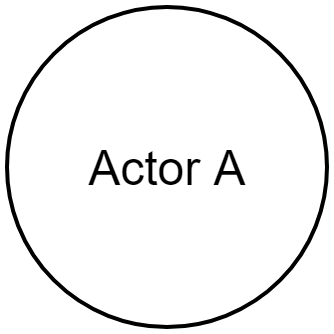
\includegraphics[width=.5\linewidth]{gfx/actor/longLiveActor}
      \captionof{figure}{Ein einfacher Actor.}
      \label{fig:test1}
    \end{minipage}%
    \begin{minipage}{.5\textwidth}
      \centering
      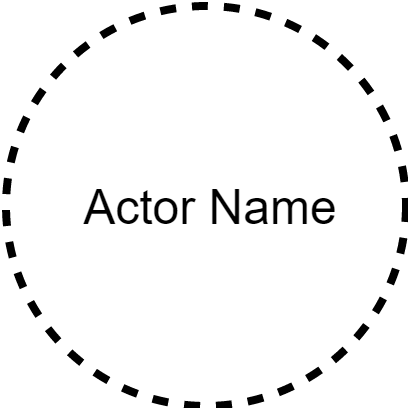
\includegraphics[width=.5\linewidth]{gfx/actor/shortLiveActor}
      \captionof{figure}{Ein Actor welcher direkt nach der Abarbeitung einer Nachricht wieder zerstört wird.}
      \label{fig:test2}
    \end{minipage}
    \end{figure}  

\subsection{Nachrichten erstellen}
Das erstellen einer Nachricht durch den Actor {A} sowie die Zustellung durch den Actor {A} and den Actor {B} wird in Abbildung~\ref{fig:actor:diagram:simpleCreateAndSendMessage} abgebildet. Wichtig ist hier, dass der Actor {A} nicht nur die Nachricht sendet, sondern sie auch erstellt!
\begin{figure}
    \centering
    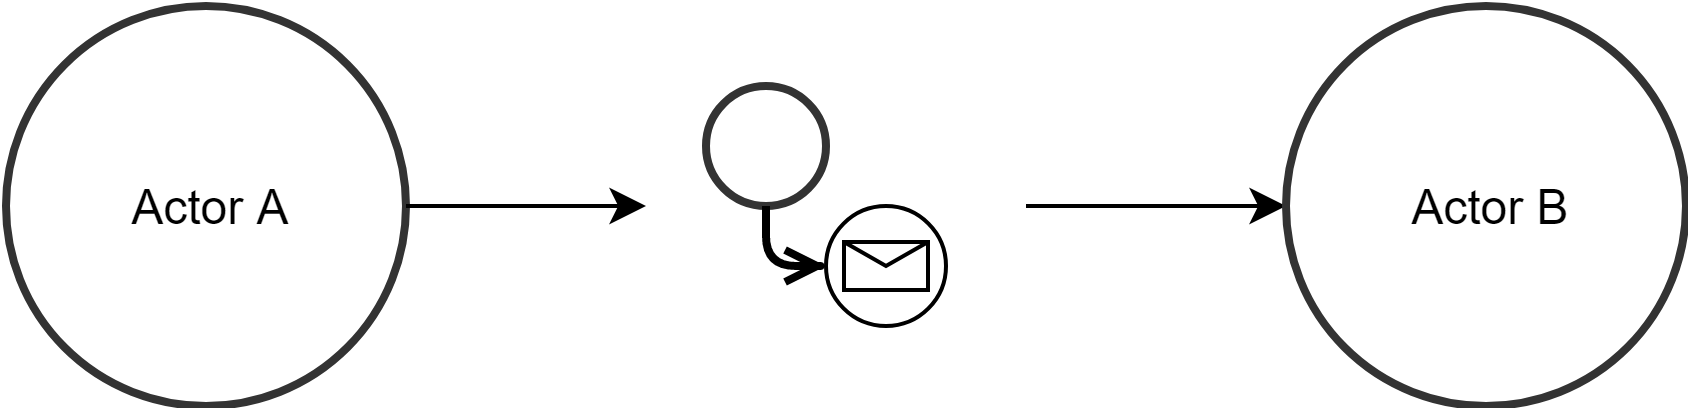
\includegraphics[width=\linewidth]{gfx/actor/simpleCreateAndSendMessage}
    \caption{Actor {A} erstellt eine neue Nachricht und sendet sie an Actor {B}.}
    \label{fig:actor:diagram:simpleCreateAndSendMessage}
\end{figure}

\subsection{Actors erstellen}
Das erstellen von Actoren durch einen Actor wird durch zwei kreise abgebildet. In Abbildung~\ref{fig:actor:diagram:childActorCreation} erstellt der {Parent}-Actor einen neuen Actor, den sogenannten {Child}-Actor.
\begin{figure}
    \centering
    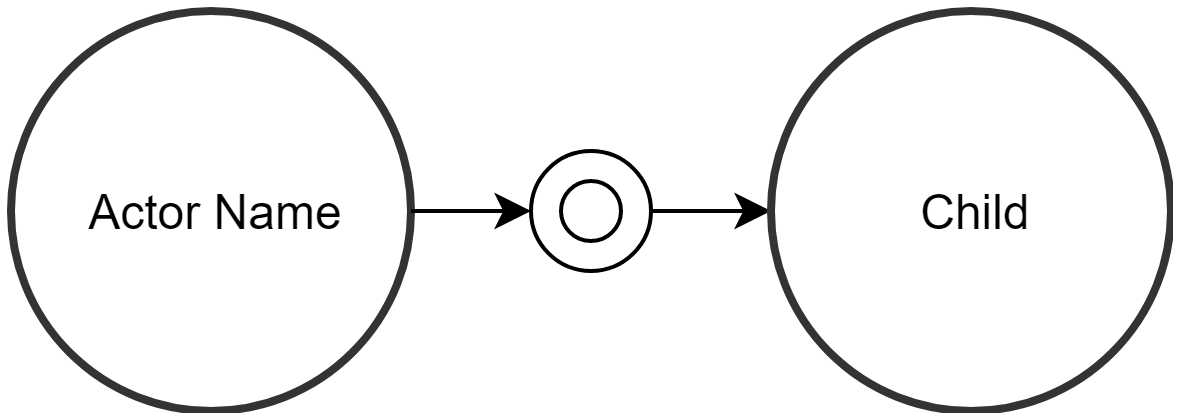
\includegraphics[width=\linewidth]{gfx/actor/childActorCreation}
    \caption{Ein Actor erstellt einen neuen Actor}
    \label{fig:actor:diagram:childActorCreation}
\end{figure}

\subsection{Darstellung eines Ablaufes}
Um einen konkreten Ablauf eines Actors darstellen zu können, benötigt man die darstellung der Nachrichteneingangsreihenfolge. Diese wird von \cite{kuhn2017reactive} und \cite{Vernon2015ReactiveAkka} als Linie dargestellt auf welcher sich Kreise befinden. Die abarbeitung wird von oben nach unten dargestellt. In Abbildung~\ref{fig:actor:diagram:asynchronMessageReceivment} bekommt der Actor zwei Nachrichten zugesendet, und sendet eine Nachricht dazwischen ab. Durch diese Abbildung ist es möglich, sequentielle Abläufe darzustellen
\begin{figure}
    \centering
    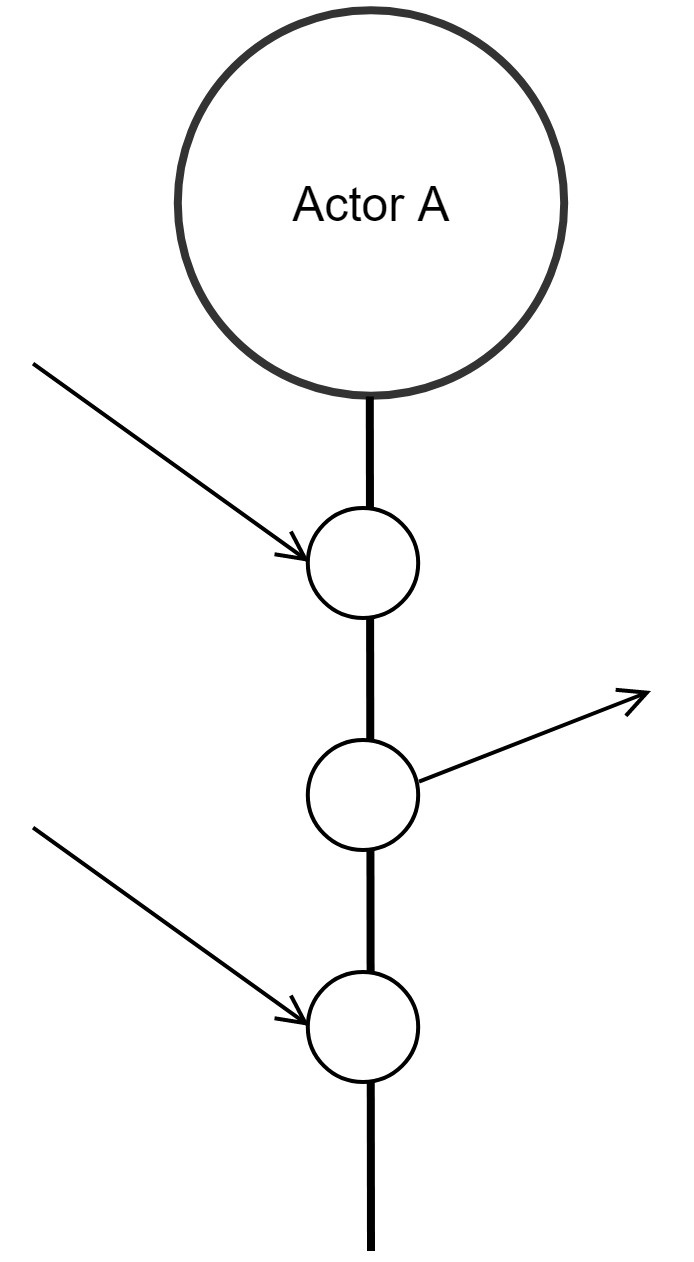
\includegraphics[height=6cm]{gfx/actor/actorAsynchMessgeFlow}
    \caption{Asynchroner Ablauf eines Actors.}
    \label{fig:actor:diagram:asynchronMessageReceivment}
\end{figure}

\section{Noch einzuordnern}
\subsection{Supervision}\label{actor:supervision}
\subsection{Location Transparent}{actor:locationTransparency}
\section{Actor basierte Architekturmuster}
\label{theory:actorArchitecture}
\section{Evaluierung}
%todo
%Agha zitate kontrollieren
\chapter{Verteilte Systeme}\label{cha:distributedSystems}
Mit dem Beginn des Computerzeitalters in den 50er Jahren galten leistungsstarke Rechner als kostenintensiv, benötigten viel Platz und operierten meist unabhängig und autark von anderen Geräten. Durch die Weiterentwicklung von Hard- und Software konnte im Laufe der Zeit diese Entwicklung von Geräten so weit gebracht werden, dass Computer heutzutage kostengünstig sowie platzsparend sind. Die Entwicklung der Netzwerktechnologien ist  weit fortgeschritten, die Vernetzung der Geräte stellt keine große Herausforderung mehr dar. Die Geräte jedoch optimal miteinander kommunizieren zu lassen, stellt Entwickler von verteilten Systemen immer wieder vor neuen Herausforderungen. \citep{tanenbaum2007distributed} \\
Dieses Kapitel soll eine Zusammenfassung über Verteile Systeme geben und deren Problematiken aufzeigen, weiters werden bekannte Lösungsvorschläge diskutiert.

\section{Definition Verteilte Systeme}\label{sec:distributedSystems:definition}
Der Begriff \textit{Verteilte Systeme} fasst eine große Anzahl an Themenblöcken zusammen, dementsprechend gibt es auch eine Vielzahl an verschiedenen Definitionen welche sich zum Teil auch voneinander grob unterscheiden. Eine weitläufige und angesehene Definition ist jene von \cite{tanenbaum2007distributed}:
\begin{quote}
    Ein verteiltes System ist eine Ansammlung von eigenständigen Rechnern die den Anwendern als ein einziges kohärentes System erscheint.
    \label{quote:distributedSystem:tanenbaum}
\end{quote}
In dieser Definition legen \cite{tanenbaum2007distributed} den Schwerpunkt auf die beteiligten Komponenten welche Computer sowie Benutzer sind. Die beteiligten Rechner arbeiten unabhängig voneinander in einem Verbund. Benutzer des Systems sehen jedoch die vernetzen Rechner nicht und müssen auch nichts darüber wissen. Für den Benutzer erscheint das verteilte System daher als ein einzelnes, zusammenhängendes System. Dadurch spürt der Benutzer zuerst keinen Unterschied, ob er mit einem einzelnen Rechner, einem Mainframe oder eben mit einem verteilten System interagiert \citep{tanenbaum2007distributed}. \\
% * <feitzinger.magdalena@gmail.com> 2018-03-06T17:11:17.068Z:
% 
% Hier ist keine Quellenangabe nötig, da du diese ja am Anfang des Satzes schon bekannt gegeben hast. 
% 
% ^.

\section{Ziele eines Verteilen Systems}\label{sec:distributedSystems:goales}
Verteilte Systeme bieten viele Vorteile und sind in einigen Bereichen von bedeutender Wichtigkeit. Jedoch ist der Einsatz eines verteilten Systems mit hohem Aufwand verbunden, weshalb nicht alle Probleme damit gelöst werden können. In \cite{tanenbaum2007distributed} werden die Ziele, welche ein Verteiltes System verfolgt, erläutert. Bei der Entscheidung ob ein Verteiltes System zur bewerkstelligen eines bestimmten Problems beiträgt, sollte das zu lösende Problem mit den folgende Zielen vereinbar sein.
% * <feitzinger.magdalena@gmail.com> 2018-03-06T17:12:52.176Z:
% 
% > Bei der Entscheidung ob ein Verteiltes System zur bewerkstelligen eines bestimmten Problems beiträgt, sollte das zu lösende Problem mit den folgende Zielen vereinbar sein.
% 
% Satz neu überdenken
% 
% ^.

\subsection{Zur Verfügungstellung von Ressourcen}\label{sec:distributedSystems:goales:resourceAccess} Das Hauptziel eines jeden Verteilten Systems ist  laut \cite{tanenbaum2007distributed} Ressourcen zu Verfügung zu stellen. Welche Art von Ressource ist unerheblich. Es kann sich um typische Web Ressourcen wie Files oder Texte handeln, oder auch physikalische Ressourcen wie beispielsweise Drucker, Scanner oder Fahrzeuge handeln.\\
Dies kann erforderlich sein um aus Kostengründen, teure Ressourcen, einer möglichst breiten Maße an Benutzern zur Verfügung zu stellen. Weiters kann der gemeinsame Zugriff auf eine oder mehrere Ressourcen zu einer besseren Zusammenarbeit zwischen verteilten Teams führen. Durch die weltweite Vernetzung durch das Internet bekommt der Zusammenbringung von verteilten Teams eine große Bedeutung zu. 
% * <feitzinger.magdalena@gmail.com> 2018-03-06T17:14:44.195Z:
% 
% > Dies
% Was ist mit dies gemeint? 
% 
% ^.
\subsection{Transparenz der Verteilung}\label{sec:distributedSystems:goales:Transperency} Wie schon aus der Definition aus Abschnitt \ref{sec:distributedSystems:definition} hervorgeht, ist ein primäres Ziel eines verteilen Systems die Transparenz des internen Aufbaues. Um Transparenz gewährleisten zu können, müssen laut \cite{iec1995open} sowie \cite{tanenbaum2007distributed} folgende Punkte in einem verteilten System erfüllt sein:
\begin{description}
    \item[Transparenter Zugang] Es ist nicht relevant wie auf eine Ressource zugegriffen wird. Bei differenzierten Zugriffsarten ist das Ergebnis sowie die Möglichkeiten der Verarbeitung der Ressource dieselbe. 
    \item[Ortsunabhängig] Eine laut \cite{tanenbaum2007distributed} bedeutende Eigenschaft der Transparenz in einem Verteilten System ist der ortsunabhängige Zugriff auf eine Ressource. Der Benutzer muss nicht den physikalischen Ort einer Ressource wissen um darauf zugreifen zu können. 
    \item[Migration] Wird eine bereits im System befindliche Ressource an einen neuen Ort verschoben, so ist diese weiterhin über die gleiche Adresse wie zuvor erreichbar.
    \item [Standortwechsel] Eine Ressource welche von einem Benutzer gerade in Verwendung ist und physikalisch an einen neuen Ort migriert wird, ist ohne Unterbrechung weiterhin für den Benutzer verwendbar.
    \item[Replizierung] Wird eine einzelne Ressource repliziert, bekommt der Verwender von dieser Replizierung nichts mit und kann diese so verwenden wie wenn die Replizierung nicht vorhanden wäre. 
    \item[Gleichzeitiger Zugriff] Eine Ressource kann unter Umständen auch von mehreren Benutzern gleichzeitig verwendet werden. Dieser gleichzeitige Zugriff ist für den einzelnen Benutzer nicht spürbar.
    \item[Fehlerresistent] Tritt bei einer Ressource ein Fehler auf, wird dieser vom User verborgen behoben oder eine andere Maßnahme ergriffen, welche dem Benutzer, so gut wie möglich, ein ungehindertes Weiterarbeiten ermöglicht.
% * <feitzinger.magdalena@gmail.com> 2018-03-06T17:39:10.033Z:
% 
% > o gut wie möglich
% ist diese erwähnung nötig? ist nur lückenfüller
% 
% ^.
\end{description}
Eine weitere Definition von \textit{Leslie Lampert} besagt, dass ein Benutzer erst merkt mit einem Verteilten System zu arbeiten, wenn ein Rechner, von dessen Existenz er bisher nichts wusste, nicht mehr funktioniert und unmittelbar Auswirkung auf seine Arbeit am System hat \citep{Schroeder:1993}. Die Definition von Lampert zeigt nochmals die Bedeutung der Transparenz für ein verteiltes System. \\
Jedoch ist in praktischen Anwendungen eine volle Transparenz für ein verteiltes System nicht immer optimal. Wie in \cite{tanenbaum2007distributed} beschrieben, sind beispielsweise transparente Zeitunterschiede in verteilten Systemen nicht immer für den Benutzer optimal. Deshalb ist eine sinnvolle Abwägung der Transparenz bestimmter Bestandteile des Systems gegenüber dem konkreten Anwendungsfall vorzunehmen. 

\subsection{Offenheit}\label{sec:distributedSystems:goales:openness} 
Ein Verteiltes System besteht in der Regel aus verschiedensten Komponenten welche untereinander sowie mit externen Teilnehmer kommunizieren. Um eine solche Kommunikation zu ermöglichen müssen Verteilte Systeme Schnittstelldefinitionen offen und standardisiert anbieten. Weiters ist es notwendig, dass ein Verteiltes System erweiterbar ist, sprich neue Komponenten während des Betriebes hinzugefügt werden können. Auch wenn neue Komponenten gänzlich andere Eigenschaften haben, wie beispielsweise Betriebssystem, Hardware etc., so ist eine Kommunikation untereinander möglich wenn sich alle beteiligten Komponenten an die definierten Schnittstellen halten. Durch diese Vorgehensweise ist ein System offen.  
% * <feitzinger.magdalena@gmail.com> 2018-03-06T17:52:32.734Z:
% 
% > wie beispielsweise Betriebssystem, Hardware etc...,
% 
% ist die Anführung eines Beispiels hier notwendig?
% 
% ^.

\subsection{Skalierung}\label{sec:distributedSystems:goales:scalability} 
Das vierte Ziel eines Verteilten Systems ist die Möglichkeit sich auf veränderte Rahmenbedingungen einzustellen. Skalierung in einem Computersystem kann laut \cite{Neuman1993Scale} in drei Dimensionen unterteilt werden. Diese sind wie folgt: 
\begin{description}
    \item[Numerisch] Die erste Dimension zielt auf die Anzahl an beteiligten Ressourcen sowie Benutzern ab. Diese variiert  und kann in einem verteilen System stark variieren.
% * <feitzinger.magdalena@gmail.com> 2018-03-06T17:54:30.065Z:
% 
% > Diese variiert  und kann in einem verteilen System stark variieren.
% 
% verwirrender satz
% 
% ^.
    \item[Geografisch] Die geografische Dimension betrachtet bei der Skalierung die geografischen Distanzen zwischen den beteiligten Komponenten. Dabei entsteht für den Benutzer kein Nachteil wenn eine Komponente hinzugefügt wird welche sich geografisch weit weg befindet.
    \item[Administrativ] In einem verteilen System können mehrere Organisationen beteiligt sein. Die administrative Dimension bei der Skalierung zeigt die beteiligten Organisationen auf welche das System betreiben.
\end{description}
Ein System ist demnach laut \cite{Neuman1993Scale} skalierbar, wenn der Anstieg an Benutzern und Ressourcen bewältigt werden kann ohne dass der Administrationsaufwand sowie die Performance des Systems darunter benachteiligt wird. \\

\subsubsection{Probleme der Skalierung}
Das Skalieren eines Systems stellt Entwickler vor immense Hürden. Häufige Problem sind laut \cite{tanenbaum2007distributed} einzelne Komponenten, welche selbst nicht skalierbar sein. Steigt nun die Anzahl an Zugriffen auf diese Komponente, kann dies zu einem Flaschenhals für das gesamte System werden. Jedoch sind unter bestimmten Umständen solche zentralisierte Komponenten nicht verhinderbar. Deshalb sollten laut \cite{tanenbaum2007distributed} diese zentralisierten Teile so gut wie möglich vom Rest des Systems entkoppelt werden. Generell sind in \cite{tanenbaum2007distributed} folgende vier Regeln angegeben, welcher ein Ablauf innerhalb eines skalierbaren, verteilen Systems erfüllen muss:
\begin{enumerate}
    \item Keine Komponente hat einen kompletten Überblick über das gesamte System
    \item Entscheidungen innerhalb einer Komponente werden nur aufgrund lokaler Informationen getroffen
    \item Ein Fehler einer einzelnen Komponente lässt den gesamten Ablauf nicht fehlschlagen
    \item Keine Entscheidung fällt aufgrund der Basis, dass es eine synchronisierte Zeit gibt
% * <feitzinger.magdalena@gmail.com> 2018-03-06T18:06:35.210Z:
% 
% > Keine Entscheidung fällt aufgrund der Basis, dass es eine synchronisierte Zeit gibt
% Satz umändern
% 
% ^.
\end{enumerate}
Der vierte und letzte Punkt ist laut \cite{tanenbaum2007distributed} deshalb nötig, weil es in einer verteilten Umgebung technisch unmöglich ist, eine Zeit exakt zu synchronisieren. Dieses Problem wird in \cite{lamport1978time} näher erläutert.\\
Die Skalierung eines Systems ist eine große Herausforderung und benötigt ein passendes, auf den Anwendungsfall angepasstes Konzept. In einem verteiltem System ist Skalierung jedoch ein äußerst wichtiges Prinzip um Anfragen effizient abarbeiten zu können.\cite{tanenbaum2007distributed}
 
\section{Limitierungen in Verteilten Systemen}
Verteilte Systeme sind aufgrund Ihrer Komplexität dementsprechend schwer umzusetzen. Bei der Realisierung eines Systems sind somit einige generell gültige Limitierungen zu berücksichtigen. Dazu gehören unter anderem die von Deutsch definierten inkorrekten Annahmen in einem verteilen System sowie das \textit{CAP-Theorem} von Brewer, welche beide nachfolgend betrachtet werden.
% * <feitzinger.magdalena@gmail.com> 2018-03-06T19:48:22.784Z:
% 
% > Deutsch
% 
% bis jetzt hast du Namen immer kursiv gehalten. warum hier nicht? 
% 
% ^.

\subsection{Die acht falschen Annahmen einer Verteilten Anwendung}\label{sec:distributedSystems:wrongAssumptions} 
Durch die Komplexität eines verteilten Systems kommt es, auch durch erfahrene Entwickler, immer wieder zu falschen Annahmen während der Konzeptionsphase. Die häufigsten fehlerhaften Annahmen wurden in \cite{deutsch1994eight} zusammengefasst. Diese Liste an fehlerhaften Grundsatzregeln sollten bei der Entwicklung eines verteilen Systems beachtet werden. Nachfolgend eine Übersicht über die acht Punkten von \cite{deutsch1994eight},, welche in \cite{rotem2006fallacies} genauer beschrieben werden.
\begin{description}
    \item[Das Netzwerk ist ausfallsicher]
    Das Verwenden eines Netzwerkes, unabhängig von der Ausführung dieses, kann immer zu Fehlern führen. Ein Netzwerk besteht laut \cite{rotem2006fallacies} aus Komponenten bei welchen plötzliche Störungen auftreten können. Daraus lässt sich ableiten, dass bei der Entwicklung eines Systems nie darauf vertraut werden kann, dass Komponenten, welche über ein Netzwerk angebunden sind, auch tatsächlich erreicht werden können. Im Architekturmuster aus Abschnitt \ref{sec:actor:patterns:guaranteedDelivery} wird dies bereits beachtet.
    \item[Das Netzwerk ist sicher]
    Informationen, welche über Netzwerke versendet werden, sind grundsätzlich nicht davor gesichert von Unbefugten gelesen zu werden. Der Verwender des Netzwerkes muss sich deshalb selbst um die Sicherheit der von ihm übertragenen Daten kümmern.
    \item[Das Netzwerk ist homogen]
    Die Bestandteile eines Netzwerkes unterscheiden sich umso mehr, je größer das Netzwerk ist. Selbst kleine Netzwerke beinhalteten meist größere Unterschiede, wie beispielsweise verschiedene Betriebssystem der Teilnehmer. Netzwerke sind deshalb nicht homogen, weshalb die Verwendung von standardisierten Protokollen wie  \textit{IP} oder \textit{XML} ratsam ist. Die nicht vorhandene Homogenität eines Netzwerkes führt laut \cite{rotem2006fallacies} meist dann zu Problemen, wenn auf proprietäre Protokolle zurückgegriffen wird.
    \item[Die Netzwerktopologie ändert sich nicht]
    Die verwendete Netzwerkinfrastruktur sowie deren Konfiguration ist laut \cite{rotem2006fallacies} nur auf den ersten Blick beständig. In einem Testszenario liegt meist die Konfiguration und der Aufbau der Infrastruktur in den Händen des Entwicklerteams. In einer Produktionsumgebung obliegt dies jedoch meist fremden Netzwerkadministratoren. Diese können Änderungen im Netzwerk vornehmen welche für die Entwickler der Anwendung nicht vorhersehbar waren. Das bedeutet, dass Entwickler einer verteilten Anwendung diese so umsetzen, dass die Anwendung selbst mögliche Änderungen des Netzwerkes unterstützt.  Beispiele hierfür sind neue Routing strecken, andere Netzwerkadressen oder der Wechsel von Netzwerkressourcen welche nicht zum Ausfall der Anwendung führen dürfen. 
    \item[Die Latenz ist null]
    Die Zeitdauer, welche vergeht bis ein Datenpaket in einem Netzwerk übertragen wird, nennt sich Latenz. Die Latenz ist aufgrund physikalischer Gesetze niemals null. Sie variiert stark, je nach dem welches Übertragungsmedium verwendet wird und welche Distanz überwunden werden soll. Eine häufige  Fehlerquellen ist \cite{rotem2006fallacies}, dass Tests und Probeläufe für ein verteiltes System unter optimalen Netzwerkbedingungen durchgeführt werden, wo die Latenz gering ist. In der Produktionsumgebung steigt jedoch dann aufgrund unterschiedlicher Faktoren die Latenz, was in weiterer folge dazu führt, dass die Anwendung in einem Fehlerzustand resultiert. 
    \item[Der Datendurchsatz ist unendlich]
    Im Gegensatz zur Latenz wird beim Datendurchsatz gemessen wie viele Daten gleichzeitig übertragen werden können. Der Datendurchsatz ist in Netzwerken ebenfalls stark begrenzt. Jedoch hat sich dieser Faktor in modernen Netzwerken laut \cite{rotem2006fallacies} in den letzten Jahren stark verbessert. Trotzdem ist der Datendurchsatz nicht unendlich und eine Verteile Anwendung muss darauf achten, welche Datenmengen über das Netzwerk übertragen werden.  
    \item[Keine Kosten bei der Datenübertragung]
    Keine Kosten bezieht sich hier einerseits auf die technischen als auch auf finanzielle Kosten. Auf technischer Seite kostet es Ressourcen, Daten in ein Netzwerk einzubringen und diese auch wieder auszulesen. So werden unter anderem Ressourcen verbraucht, Daten zu serialisieren sowie die Verbindung zum Netzwerk aufzubauen und auch diese zu halten. Weiters benötigt die Erstellung sowie die Erhaltung eines Netwerkes finanzielle Ressourcen, welche je nach Größe des Netzwerkes beachtlich sein können \cite{rotem2006fallacies}.
    \item[Es gibt nur einen Administrator]
    Wird eine Anwendung in einer größeren Umgebung ausgerollt, so sind auch mehr Personen daran beteiligt. Auch die Administration eines Netzwerkes kann dann unterschiedlichen Personen obliegen. Vor allem wenn die Umgebung, in welchem die Anwendung läuft, zwischen mehreren Organisationen aufgeteilt ist. Meist sind diese Personen auch nicht an der Entwicklung der Anwendung beteiligt. Deshalb ist es erforderlich, Verwaltungstools oder ähnliches für diese Gruppe an Netzwerkadministratoren anzubieten, damit diese einen Überblick über die Anwendung bekommen \cite{rotem2006fallacies}.  
\end{description}
Diese acht Annahmen sind trotz ihres Alters auch heute noch wichtig und sollten von Architekten für verteilte Systeme immer wieder beachtet werden. Auch wenn die Regeln meist logisch und klar erscheinen werden sie in der Praxis immer wieder, aufgrund unterschiedlichster Gründe, gebrochen. \cite{rotem2006fallacies} 

\section{CAP-Theorem}\label{sec:distributedSystems:capTheorem}
Eine weitere bedeutende Limitierung innerhalb eines verteilten System stellt das \textit{CAP-Theorem}  dar. Das von Eric Brewer in \cite{Brewer2000TowardsSystems}  erstmals beschriebene Theorem beschreibt die Limitierung von drei gewünschten Eigenschaften in einem verteilen System. Diese drei Eigenschaften sind Konsistenz, Verfügbarkeit sowie Partition Toleranz. Nach dem \textit{CAP-Theorem} können in jedem System nur zwei der drei Eigenschaften garantiert werden. Auf eine der drei Eigenschaften muss auf jeden Fall verzichtet werden. In \cite{gilbertPerspectiveCAPTheorem2012} wird das \textit{CAP-Theorem} mit dem aktuellen Stand der Dinge wie folgt beschrieben.

\begin{description}
\item[Konsistenz]
Die Konsistenz der Daten, welche ein verteiltes System als Antwort an Anfragen gibt, sollte gegeben sein. Das ist je nach Komplexitätsgrad der Anwendung unterschiedlich möglich. So ist laut \cite{gilbertPerspectiveCAPTheorem2012} der Koordinationsaufwand für die Erstellung der Daten ausschlaggebend für die Erhaltung der Konsistenz eines Systems. Können die Daten aufgrund von statischen Berechnungen erzeugt werden, ist die Konsistenz wesentlich leichter zu realisieren, als wenn die Daten über das gesamte Netzwerk verteilt werden müssen. Ein verteiltes System ist dann Konsistenz, wenn sichergestellt ist, dass jede beteiligte Komponente den gleichen Datenbestand sehen kann und somit keine Inkonsistenzen entstehen können.   

\item[Verfügbarkeit]
Die Verfügbarkeit eines Systems, wie bereits im {\textit{Reactive Manifesto}} in Kapitel \ref{reactivo:responsive} gefordert, bedeutet, dass das System zu jeder Zeit ankommende Anfragen beantworten kann. Die Antwort muss dabei innerhalb einer, zum Kontext der Aufgabe vertretbaren Zeit, erfolgen.

\item[Partition Toleranz]
Da das verteilte System aus mehreren beteiligten Komponenten besteht, müssen diese auch miteinander kommunizieren. Weil wie bereits in Abschnitt \ref{sec:distributedSystems:wrongAssumptions} besprochen, die Kommunikation in einem System nie garantiert werden kann, können durch Verbindungsunterbrechungen im Netzwerk Partitionen entstehen. Partitioniert sich ein Netzwerk, ist die Kommunikation zwischen den entstandenen Partitionen temporär nicht mehr möglich.
\end{description}
Eine Regel, das in einem verteilten System eben nur zwei der drei genannten Kriterien gleichzeitig gewährleistet werden kann, führt dazu, dass man sich, abwiegend auf Basis des Anwendungsfall, von einer der drei Eigenschaften trennen muss. Dies kann jedoch oft durch organisatorische Prozesse abgedeckt werden, was jedoch nichts mit dem \textit{CAP-Theorem} zu tun hat. Bei einem Ausfallsicheren verteilten System ist Partition Toleranz auf jeden Fall Voraussetzung, da sich das Netzwerk jederzeit partitionieren kann. Jedoch ist auch hier wieder die optimale Zusammensetzung der drei \textit{CAP}-Parameter von der konkret umzusetzenden Thematik abhängig. Um beispielsweise einen Kompromiss mit der Konsistenz der Daten zu erhalten bietet sich das in Kapitel \ref{sec:transactionTheory:base} beschriebene \textit{BASE-Prinzip} an.
\chapter{Transaktionssysteme}
\chapter{Evaluierung}
\section{Alternative Methodiken}
\section{Das Actor Model zur Realisierung von verteilten, Transaktionssystemen} 
\section{Forschungsfrage} 


\cleardoublepage\part{Praktische Umsetzung}

\chapter{Eruierung für ein verteiltes Transaktionalen Actor System }
\section{Forschungsmethodik Einführung in das Praxisbeispiel (Flugbuchungssystem)}
\section{Actor Frameworks}\label{sec:ActorFrameworks}
Welche Möglichkeiten gibt es das Actor Model in der Praxis zu verwenden (Scala, Akka, Akka.Net, Orleans usw)

\section{Anforderungskatalog}
Anhand des theoretischen Teiles soll ein Anforderungskatalog für eine praktische Umsetzung erstellt werden.

\section{Testdaten}

\chapter{Umsetzung eines Verteilen Transaktionalen Systemes mit dem Actor Model}
Wie wurde die praktische Implementierung Umgesetzt um den Anforderungskatalog zu erfüllen. Warum wurde welche Technologie gewählt? Welche Probleme gibt es? 

\chapter{Evaluierung}
\section{Auseinandersetzung mit der Forschungsfrage}
\section{Bewertung der Umsetzung}
\section{Weiterführende Diskussionen und Forschungsausblick}


% ********************************************************************
% Backmatter
% ********************************************************************
\appendix
% insert your appendix here

%%************************************************
\chapter{Introduction to the ClassicThesis style}\label{ch:introduction}
%************************************************
This bundle for \LaTeX\ has two goals:
\begin{enumerate}
    \item Provide students with an easy-to-use template for their
    Master's
    or PhD thesis. (Though it might also be used by other types of
    authors
    for reports, books, etc.)
    \item Provide a classic, high quality typographic style which is
    inspired by \citeauthor{bringhurst:2002}'s ``\emph{The Elements of
    Typographic Style}'' \citep{bringhurst:2002}.
    \graffito{\myTitle \myVersion}
\end{enumerate}
The bundle is configured to run with a \emph{full} 
MiK\TeX\ or \TeX Live\footnote{See the file \texttt{LISTOFFILES} for
needed packages. Furthermore, \texttt{classicthesis} 
works with most other distributions and, thus, with most operating 
systems \LaTeX\ is available for.} 
installation right away and, therefore, it uses only freely available 
fonts. (Minion fans can easily adjust the style to their needs.)

People interested only in the nice style and not the whole bundle can
now use the style stand-alone via the file \texttt{classicthesis.sty}.
This works now also with ``plain'' \LaTeX.

This should enable anyone with a basic knowledge of \LaTeXe\ to
produce beautiful documents without too much effort. In the end, this
is my overall goal: more beautiful documents, especially theses, as I
am tired of seeing so many ugly ones.

The whole template and the used style is released under the
\textsmaller{GNU} General Public License. 

If you like the style then I would appreciate a postcard:
\begin{center}
 Andre Miede \\
 Detmolder Strasse 32 \\
 31737 Rinteln \\
 Germany
\end{center}
The postcards I got so far are available at \url{http://postcards.miede.de}.

Hopefully, this thesis template is done well enough for your needs and
does not have too many flaws. So far, a couple of theses have been
typeset successfully with it. If you are interested in some
typographic details behind it, enjoy Robert Bringhurst's wonderful book.

\graffito{A well-balanced line width improves the legibility of
the text. That's what typography is all about, right?}
\paragraph{Important Note:} Some things of this style might look
unusual at first glance, many people feel so in the beginning.
However, all things are intentionally designed to be as they are,
especially these:
\begin{itemize}
    \item No bold fonts are used. Italics or spaced small caps do the
    job quite well.
    \item The size of the text body is intentionally shaped like it
    is. It supports both legibility and allows a reasonable amount of
    information to be on a page. And, no: the lines are not too short.
    \item The tables intentionally do not use vertical or double
    rules. See the documentation for the \texttt{booktabs} package for
    a nice discussion of this topic.\footnote{To be found online at \\
    \url{http://www.ctan.org/tex-archive/macros/latex/contrib/booktabs/}.}
    \item And last but not least, to provide the reader with a way
    easier access to page numbers in the table of contents, the page
    numbers are right behind the titles. Yes, they are \emph{not}
    neatly aligned at the right side and they are \emph{not} connected
    with dots that help the eye to bridge a distance that is not
    necessary. If you are still not convinced: is your reader
    interested in the page number or does she want to sum the numbers
    up?
\end{itemize}
Therefore, please do not break the beauty of the style by changing
these things unless you really know what you are doing! Please.


\section{Organization}
A very important factor for successful thesis writing is the
organization of the material. This template suggests a structure as
the following:
\begin{itemize}
    \graffito{You can use these margins for summaries of the text
    body\dots}
    \item\texttt{Chapters/} is where all the ``real'' content goes in
    separate files such as \texttt{Chapter01.tex} etc.
 %  \item\texttt{Examples/} is where you store all listings and other
 %  examples you want to use for your text.
    \item\texttt{FrontBackMatter/} is where all the stuff goes that
    surrounds the ``real'' content, such as the acknowledgments,
    dedication, etc.
    \item\texttt{gfx/} is where you put all the graphics you use in
    the thesis. Maybe they should be organized into subfolders
    depending on the chapter they are used in, if you have a lot of
    graphics.
    \item\texttt{Bibliography.bib}: the Bib\TeX\ database to organize
    all the references you might want to cite.
    \item\texttt{classicthesis.sty}: the style definition to get this
    awesome look and feel. 
    \item\texttt{ClassicThesis.tcp} a \TeX nicCenter project file.
    Great tool and it's free!
    \item\texttt{ClassicThesis.tex}: the main file of your thesis
    where all gets bundled together.
    \item\texttt{classicthesis-ldpkg.sty}: a central place to load all 
    nifty packages that are used. The package has the following options 
    available:
		\begin{itemize}
			\item\texttt{nochapters}, which defaults to \texttt{false}.
		    Activate it if you want to use the package with a class which does
		    not have chapter divisions, \eg, an article.
		    \item\texttt{backref}, which also defaults to \texttt{false}.
		    Activate it if you do want to show in the bibliography on which
		    page(s) each reference was cited. %See page~\pageref{app:bibliography} 
		    for an example of the default setting.
		\end{itemize}
\end{itemize}
This should get you started in no time.


\section{Style Options}
There are a couple of options for \texttt{classicthesis.sty} that
allow for a bit of freedom concerning the layout:
\begin{itemize}
    \graffito{\dots or your supervisor might use the margins for some
    comments of her own while reading.}
    \item\texttt{drafting}: prints the date and time at the bottom of
    each page, so you always know which version you are dealing with.
    Might come in handy not to give your Prof. that old draft.
    \item\texttt{eulerchapternumbers}: use figures from Hermann Zapf's
    Euler math font for the chapter numbers. By default, old style
    figures from the Palatino font are used.
    \item\texttt{linedheaders}: changes the look of the chapter
    headings a bit by adding a horizontal line above the chapter
    title. The chapter number will also be moved to the top of the
    page, above the chapter title.
    \item\texttt{listsseparated}: will add extra space between table
    and figure entries of different chapters in the list of tables or
    figures, respectively.
    \item\texttt{tocaligned}: aligns the whole table of contents on
    the left side. Some people like that, some don't.
    \item\texttt{subfig}(\texttt{ure}): is passed to the \texttt{tocloft} 
    package to enable compatibility with the \texttt{subfig}(\texttt{ure}) 
    package.
    \item\texttt{nochapters}: allows to use the look-and-feel with 
    classes that do not use chapters, \eg, for articles. Automatically
    turns off a couple of other options: \texttt{eulerchapternumbers}, 
    \texttt{linedheaders}, \texttt{listsseparated}, and \texttt{parts}.
    \item\texttt{beramono}: loads Bera Mono as typewriter font. 
    (Default setting is using the standard CM typewriter font.)
    \item\texttt{eulermath}: loads the awesome Euler fonts for math. 
    (Palatino is used as default font.)
    \item\texttt{parts}: if you use Part divisions for your document,
    you should choose this option. It provides you with the command
    \verb|\myPart{}| which takes care of the style and the entry
    into the Table of Contents. (Cannot be used together with
    \texttt{nochapters}.)
    \item\texttt{a5paper}: adjusts the page layout according to the
    global \texttt{a5paper} option (\emph{experimental} feature).
    \item\texttt{minionpro}: sets Robert Slimbach's Minion as the 
    main font of the document. The textblock size is adjusted 
    accordingly. 
    \item\texttt{pdfspacing}: makes use of pdftex' letter spacing
    capabilities via the \texttt{microtype} package.\footnote{Use 
    \texttt{microtype}'s \texttt{DVIoutput} option to generate
    DVI with pdftex.} This fixes some serious issues regarding 
    math formul\ae\ etc. (\eg, ``\ss'') in headers. 
    \item\texttt{minionprospacing}: uses the internal \texttt{textssc}
    command of the \texttt{MinionPro} package for letter spacing. This 
    automatically enables the \texttt{minionpro} option and overrides
    the \texttt{pdfspacing} option.
    \item\texttt{dottedtoc}: sets pagenumbers flushed right in the 
    table of contents.
    \item\texttt{listings}: loads the \texttt{listings} package (if not 
    already done) and configures the List of Listings accordingly.
    \item\texttt{manychapters}: if you need more than nine chapters for 
    your document, you might not be happy with the spacing between the 
    chapter number and the chapter title in the Table of Contents. 
    This option allows for additional space in this context. 
    However, it does not look as ``perfect'' if you use
    \verb|\parts| for structuring your document.
\end{itemize}
The best way to figure these options out is to try the different
possibilities and see, what you and your supervisor like best.

To make things in general easier, \texttt{classicthesis-ldpkg.sty} 
contains some useful commands that might help you.


\section{Future Work}
So far, this is a quite stable version that served a couple of people
well during their thesis time. However, some things are still not as
they should be. Proper documentation in the standard format is still
missing. In the long run, the style should probably be published
separately, with the template bundle being only an application of the
style. Alas, there is no time for that at the moment\dots it could be
a nice task for a small group of \LaTeX nicians.

Please do not send me email with questions concerning \LaTeX\ or the
template, as I do not have time for an answer. But if you have
comments, suggestions, or improvements for the style or the template
in general, do not hesitate to write them on that postcard of yours.


\section{License}
\paragraph{GNU General Public License:} This program is free software;
you can redistribute it and/or modify
 it under the terms of the \textsmaller{GNU} General Public License as
 published by
 the Free Software Foundation; either version 2 of the License, or
 (at your option) any later version.

 This program is distributed in the hope that it will be useful,
 but \emph{without any warranty}; without even the implied warranty of
 \emph{merchantability} or \emph{fitness for a particular purpose}.
 See the
 \textsmaller{GNU} General Public License for more details.

 You should have received a copy of the \textsmaller{GNU} General
 Public License
 along with this program; see the file \texttt{COPYING}.  If not,
 write to
 the Free Software Foundation, Inc., 59 Temple Place - Suite 330,
 Boston, \textsmaller{MA} 02111-1307, \textsmaller{USA}.


\section{Beyond a Thesis}
It is easy to use the layout of \texttt{classicthesis.sty} without the
framework of this bundle. To make it even easier, this section offers 
some plug-and-play-examples.

%*****************************************
%*****************************************
%*****************************************
%*****************************************
%*****************************************






%********************************************************************
% Other Stuff in the Back
% ********************************************************************´
\cleardoublepage%********************************************************************
% Bibliography
%*******************************************************
% work-around to have small caps also here in the headline
\manualmark
\markboth{\spacedlowsmallcaps{\bibname}}{\spacedlowsmallcaps{\bibname}} % work-around to have small caps also
%\phantomsection 
\refstepcounter{dummy}
\addtocontents{toc}{\protect\vspace{\beforebibskip}} % to have the bib a bit from the rest in the toc
\addcontentsline{toc}{chapter}{\tocEntry{\bibname}}

\bibliographystyle{apa} 
\label{app:bibliography} 
\bibliography{IEEEabrv,Bibliography}



% ********************************************************************
% Game Over: Restore, Restart, or Quit?
% ********************************************************************
\end{document}
% ********************************************************************
